\part{监督学习}

不妨先从监督学习的几个例子谈起。假设有一个记录了俄勒冈州波特兰市 47 套房屋的居住面积和价格的数据集:

\begin{table}[h]
    \centering
    \begin{tabular}{c|c}
        居住面积 (平方英尺) & 价格 (1000\$) \\
        \hline
        2104 & 400 \\
        1600 & 330 \\
        2400 & 369 \\
        1416 & 232 \\
        3000 & 540 \\
        $\vdots$ & $\vdots$
    \end{tabular}
    \label{tab:house_example}
\end{table}

将这些数据绘制出来:

\begin{figure}[H]
    \centering
    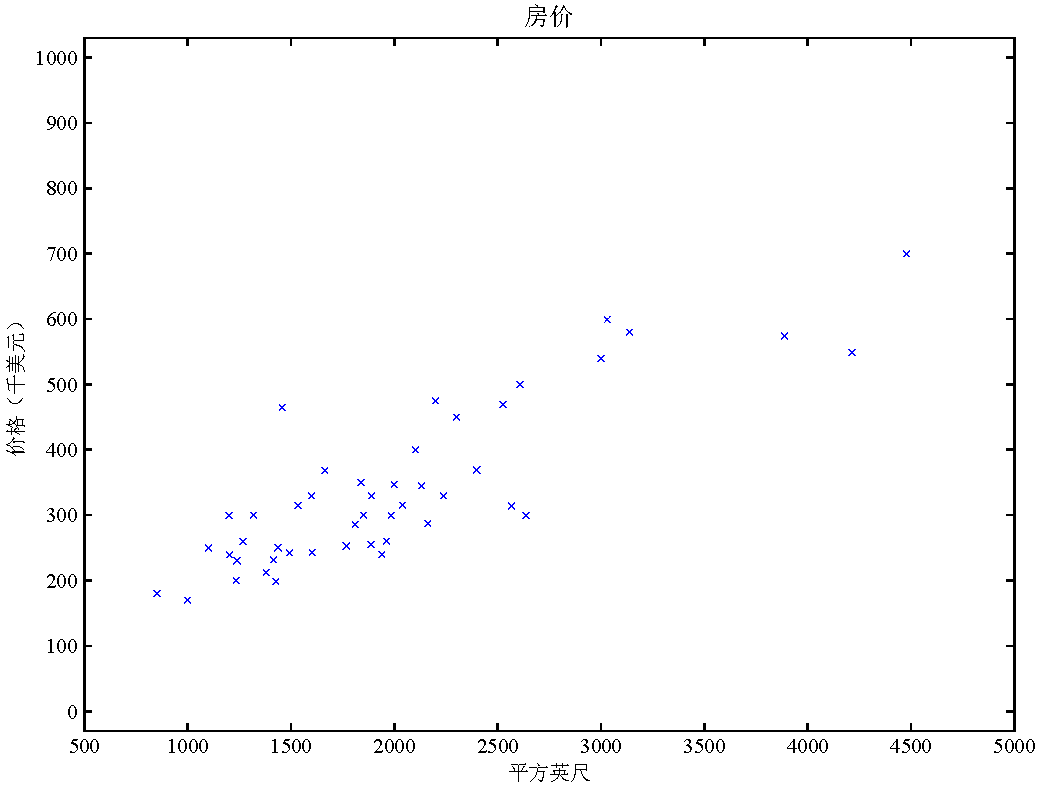
\includegraphics[width=0.5\linewidth]{figs/house_dataset_plot1.pdf}
\end{figure}

有了这些数据之后,该怎样根据波特兰其他房屋的居住面积来预测其价格呢?

为了后续使用的方便,在这里做如下约定。约定用 $x^{(i)}$ 表示“输入”变量(示例中是居住面积),也称作输入\textbf{特征 (features)};用 $y^{(i)}$ 表示要预测的“输出”或\textbf{目标 (target) }变量(价格)。一对 $(x^{(i)}, y^{(i)})$ 称为一个\textbf{训练样本 (training example)},而用于学习的数据集——由 $n$ 个训练样本组成的列表 $\{(x^{(i)}, y^{(i)}); i = 1,...,n\}$——则称为\textbf{训练集 (training set)}。注意,此处的上标“$i$”仅表示训练集中的索引,而不表示指数运算。此外,用 $\mathcal{X}$ 表示输入的取值空间,$\mathcal{Y}$ 表示输出的取值空间。在本例中,有 $\mathcal{X} = \mathcal{Y} = \mathbb{R}$。

监督学习问题可以更加形式化地表述为:给定一个训练集,目标是学习一个函数 $h: \mathcal{X} \mapsto \mathcal{Y}$,该函数能够对输入 $x$ 进行预测,使其输出 $h(x)$ 与“很好地”预测相应的真实值 $y$。出于历史原因,函数 $h$ 被称为 \textbf{假设 (hypothesis)}。整个过程如下图所示:

\begin{figure}[H]
\centering
\begin{tikzpicture}[node distance=2cm, auto]
    \node [rounded corners=1mm, rectangle, align=center, draw] (training) {训练集};
    \node [rounded corners=1mm, rectangle, align=center, draw, below of=training] (learning) {学习算法};
    \node [rounded corners=1mm, rectangle, align=center, draw, below of=learning] (h) {$h$};
    \node [left of=h, label={[align=center]below:\footnotesize (房屋居住面积)}] (x) {$x$};
    \node [right of=h, label={[align=center]below:\footnotesize (房屋预测价格)}] (y) {预测值 $y$};

    \path [->, draw] (training) -- (learning);
    \path [->, draw] (learning) -- (h);
    \path [->, draw] (x) -- (h);
    \path [->, draw] (h) -- (y);
\end{tikzpicture}
\end{figure}

当预测的目标变量是连续值时(例如预测房价),称这类学习问题为\textbf{回归 (regression)} 问题。当 $y$ 只能取有限个离散值时(例如根据居住面积预测住宅是房屋还是公寓),则称为\textbf{分类 (classification)} 问题。

\chapter{线性回归}

为了让上面的房屋示例更有趣,不妨考虑一个更为丰富的数据集。除了居住面积外,该数据集还包括了每栋房屋的卧室数量:

\begin{table}[H]
    \centering
    \begin{tabular}{c|c|c}
        居住面积 (平方英尺) & 卧室数 & 价格 (1000\$) \\
        \hline
        2104 & 3 & 400 \\
        1600 & 3 & 330 \\
        2400 & 3 & 369 \\
        1416 & 2 & 232 \\
        3000 & 4 & 540 \\
        $\vdots$ & $\vdots$ & $\vdots$
    \end{tabular}
    \label{tab:house_example2}
\end{table}

此处,$x$ 是 $\mathbb{R}^2$ 中的二维向量。对于训练集中第 $i$ 栋房屋,$x_1^{(i)}$ 是其居住面积,而 $x_2^{(i)}$ 是其卧室数量。(在设计学习问题时,特征的选择通常取决于你的具体需求。例如,在收集波特兰的房屋数据时,除了居住面积和卧室数量,还可以考虑纳入壁炉、浴室数量等其他特征。关于特征选择的深入讨论将在后续展开,目前先基于当前给定的两个特征进行分析。)

在进行监督学习时,需要明确如何在计算机中表示假设函数 $h$。不妨先尝试用 $x$ 的线性函数来近似 $y$:

\[
    h_\theta(x) = \theta_0 + \theta_1x_1 + \theta_2x_2
\]
在此处,$\theta_i$ 是该模型的\textbf{参数 (parameters)},亦称\textbf{权重 (weights)}。它们参数化了从特征空间 $\mathcal{X}$ 到目标空间 $\mathcal{Y}$ 的线性函数。在不引起混淆的前提下,可以省略 $h_\theta(x)$ 中的下标 $\theta$,直接写作 $h(x)$。为了进一步简化表示,我们引入约定:令 $x_0 = 1$。这个 $x_0$ 对应的系数 $\theta_0$ 通常被称为\textbf{截距项 (intercept term)}。这样就有

\[
    h(x) = \sum_{i=0}^d \theta_i x_i = \theta^T x,
\]
其中 $\theta$ 和 $x$ 视为向量,而 $d$ 则是输入变量的数量 (不计入 $x_0$)。

现在,对于给定的训练集,我们应该如何选择或学习参数 $\theta$ 呢?一个直观且合理的方法是,使假设函数 $h(x)$ 对于训练样本的输出 $h_\theta(x^{(i)})$ 尽可能地接近其对应的真实值 $y^{(i)}$。为了形式化地表述这个接近程度,我们定义一个函数,用于衡量对于任意给定的参数值 $\theta$,预测值 $h_\theta(x^{(i)})$ 与实际值 $y^{(i)}$ 之间的差异。这个函数被称为\textbf{代价函数 (cost function)}:

\[
    J(\theta) = \frac{1}{2} \sum_{i=1}^n (h_\theta(x^{(i)}) - y^{(i)})^2.
\]

熟悉线性回归的读者可能会发现,此处定义的函数即为\textbf{普通最小二乘 (ordinary least squares)} 回归模型所使用的最小二乘代价函数。但本讲义不要求读者具备相关背景知识,后文将对此进行详细阐述,并最终指出这仅是更广泛算法族中的一个特例。


\section{最小均方算法}

我们的目标是找到能够最小化代价函数 $J(\theta)$ 的参数 $\theta$。为此,我们可以考虑一种搜索算法:该算法从对 $\theta$ 的某个“初始猜测”开始,然后不断地调整 $\theta$ 的值,使其沿着使 $J(\theta)$ 减小的方向移动,直到最终收敛到最小化 $J(\theta)$ 的 $\theta$ 值。具体而言,我们考虑使用\textbf{梯度下降 (gradient descent)} 算法。该算法从某个初始的 $\theta$ 值开始,并重复执行以下更新步骤:

\[
    \theta_j := \theta_j - \alpha \frac{\partial}{\partial\theta_j} J(\theta).
\]
(上述更新操作同时应用于 $j = 0, \dots, d$ 的所有参数 $\theta_j$。)这里的 $\alpha$ 被称为\textbf{学习率 (learning rate)}。这是一种非常自然的算法:它每一步都沿着代价函数 $J$ 下降最快的方向进行更新。

为了实现上述算法,需要计算公式右侧的偏导数项。可以先考虑只有一个训练样本 $(x, y)$ 的情况,这样就可以暂时忽略代价函数 $J$ 定义中的求和操作。在这种情况下,偏导数计算如下:

\[
    \begin{aligned}
    \frac{\partial}{\partial\theta_j} J(\theta) &= \frac{\partial}{\partial\theta_j} \frac{1}{2} (h_\theta(x) - y)^2 \\
    &= 2 \cdot \frac{1}{2} (h_\theta(x) - y) \cdot \frac{\partial}{\partial\theta_j} (h_\theta(x) - y) \\
    &= (h_\theta(x) - y) \cdot \frac{\partial}{\partial\theta_j} \left( \sum_{i=0}^d \theta_i x_i - y \right) \\
    &= (h_\theta(x) - y) x_j
    \end{aligned}
\]

上式给出了针对单个训练样本的更新规则:\footnote{符号 “$a := b$” 用于表示(计算机程序中的)一个操作,其中变量 $a$ 的值被设置为 $b$。换句话说,这个操作用 $b$ 的值覆盖了 $a$ 的值。反之,如果需要断言 $a$ 的值等于 $b$ 的值,会写作 “$a = b$”。}

\[
    \theta_j := \theta_j + \alpha (y^{(i)} - h_\theta(x^{(i)})) x_j^{(i)}.
\]
这个规则被称为\textbf{最小均方 (Least mean squares, LMS)} 更新规则,也称为 \textbf{Widrow-Hoff} 学习规则。该规则具有一些自然而直观的特性。例如,更新的幅度与\textbf{误差 (error)} 项 $(y^{(i)} - h_\theta(x^{(i)}))$ 成正比;因此,如果对于一个训练样本,其预测值几乎等于 $y^{(i)}$ 的实际值,那么参数就几乎不需要调整;反之,如果预测的 $h_\theta(x^{(i)})$ 有很大的误差 (即与 $y^{(i)}$ 相差甚远),则需要对参数进行更大的调整。

所推导的 LMS 规则是针对只有一个训练样本的情况。要将其应用于包含多个样本的训练集,有两种常见的方法。第一种方法是将算法修改为以下形式:

\vspace{0.5em}
重复直到收敛 \{
\begin{equation}
    \theta_j := \theta_j + \alpha \sum_{i=1}^n (y^{(i)} - h_\theta(x^{(i)})) x_j^{(i)}, \text{(对于每个 } j) \label{eq:1.1}
\end{equation}
\indent\}
\vspace{0.5em}

将逐位置的更新向量化到 $\theta$,可以稍微简化 \eqref{eq:1.1}:

\[
    \theta := \theta + \alpha \sum_{i=1}^n (y^{(i)} - h_\theta(x^{(i)})) x^{(i)}
\]

读者不难验证,上述更新规则中求和项所表示的量,恰好对应于我们先前定义的成本函数的偏导数 $\partial J(\theta) / \partial \theta_j$。因此,这个更新规则实际上就是在原始成本函数 $J$ 上进行梯度下降。这种方法在每一步都利用了整个训练集的所有样本,因此被称为\textbf{批量梯度下降 (batch gradient descent)}。值得注意的是,尽管梯度下降算法在一般情况下可能收敛到局部最优解,但对于我们这里的线性回归问题,其优化目标函数 $J$ 具有良好的性质:它是一个凸二次函数。这意味着它只有一个全局最小值,没有其他局部最优解。因此,在合适的学习率 $\alpha$ 下,梯度下降算法能够保证收敛到全局最优解。下面是一个用梯度下降最小化一个二次函数的图例。

\begin{figure}[H]
    \centering
    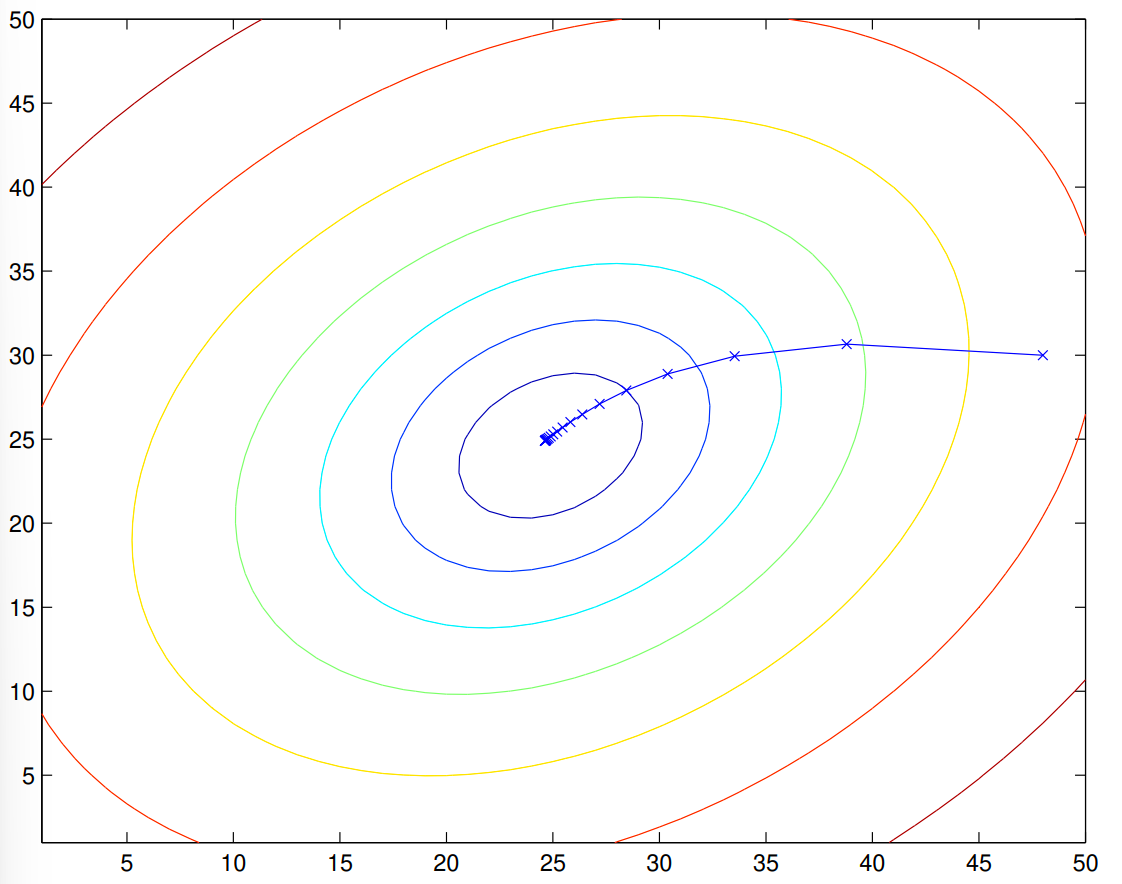
\includegraphics[width=0.5\linewidth]{figs/gradient_descent_trajectory.png}
    \label{fig:gradient_descent_trajectory}
\end{figure}
上面的椭圆是二次函数的等高线。图中还显示了梯度下降的轨迹,其初始化参数是 (48,30),而由直线连接的叉号 $\text{x}$ 则是梯度下降所经过的一系列参数 $\theta$ 值。

在之前的数据集上应用批量梯度下降算法来拟合参数 $\theta$,以学习根据居住面积预测房价的函数,最终得到的参数值为 $\theta_0 = 71.27$ 和 $\theta_1 = 0.1345$。将学习到的函数 $h_\theta(x)$,作为输入变量 $x$(表示居住面积)的函数,与训练数据一同绘制,结果如下图所示:

\begin{figure}[H]
    \centering
    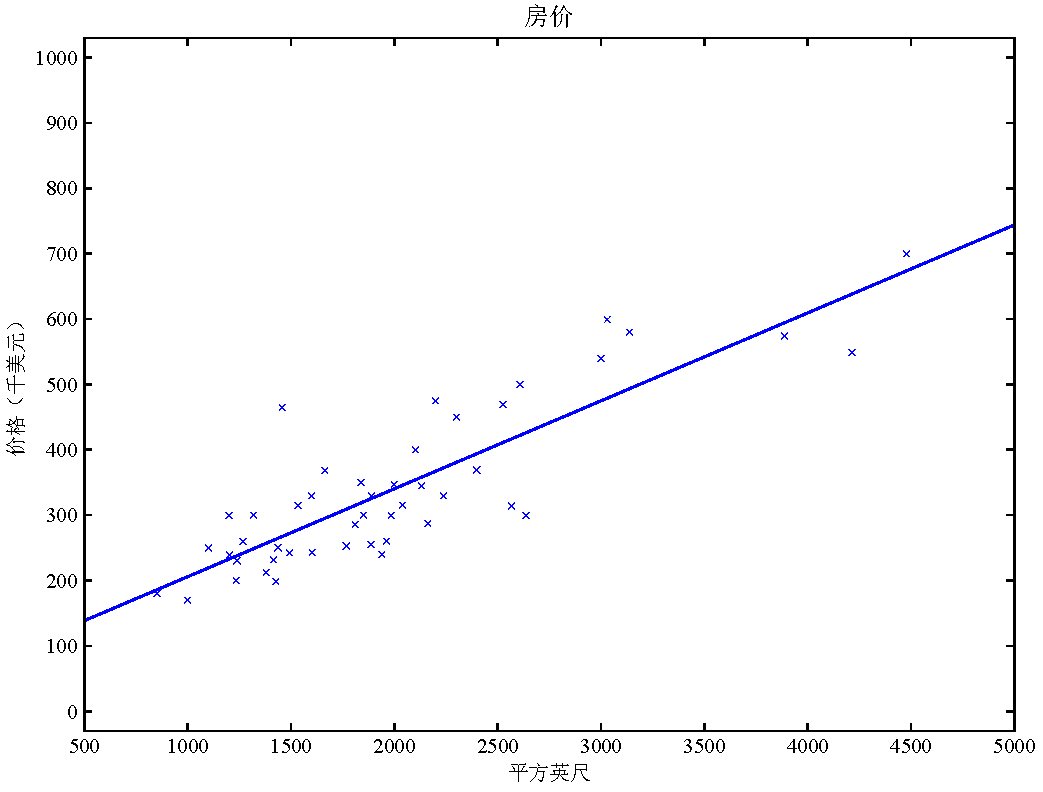
\includegraphics[width=0.5\linewidth]{figs/house_dataset_plot2.pdf}
\end{figure}
如果把卧室数量也当作输入特征,最终得到的参数值为 $\theta_0 = 89.60, \theta_1 = 0.1392, \theta_2 = -8.738$。

上述结果是通过批量梯度下降算法得到的。除此之外,还有一种很好的替代算法:

\vspace{0.5em}
循环 \{

$\quad\quad$对于 $i = 1$ 到 $n$,\{

\begin{equation}
    \theta_j := \theta_j + \alpha (y^{(i)} - h_\theta(x^{(i)})) x_j^{(i)}, \text{(对于每个 } j) \label{eq:1.2}
\end{equation}

$\quad\quad$\}

\indent\}
\vspace{0.5em}

将逐位置的更新向量化到 $\theta$,可以稍微简化 \eqref{eq:1.2}:

\[
    \theta := \theta + \alpha (y^{(i)} - h_\theta(x^{(i)})) x^{(i)}
\]

这种算法会重复遍历训练集,每次遇到一个训练样本时,仅针对该单个样本计算误差梯度并更新参数。这种方法被称为\textbf{随机梯度下降 (stochastic gradient descent)},有时也称为\textbf{增量梯度下降 (incremental gradient descent)}。与批量梯度下降不同,批量梯度下降在执行单次更新前需要扫描整个训练集(当训练集规模 $n$ 很大时,这是一项昂贵的操作),而随机梯度下降可以立即开始并对每个样本都取得进展。通常情况下,随机梯度下降能更快地使参数 $\theta$ “接近”最小值。(然而,需要注意的是,它可能不会完全“收敛”到最小值,参数 $\theta$ 可能会在目标函数 $J(\theta)$ 的最小值附近持续振荡。但在实际应用中,接近最小值的大多数值都足以作为真实最小值的良好近似。\footnote{通过在算法运行过程中缓慢地减小学习率 $\alpha$ 至零,可以确保参数收敛到全局最小值,而不仅仅是在最小值附近振荡。} )因此,特别是在训练集很大时,通常更倾向于使用随机梯度下降而非批量梯度下降。


\section{正规方程}

梯度下降提供了一种最小化目标函数 $J$ 的迭代方法。接下来,我们将探讨另一种无需迭代的最小化 $J$ 的方法。具体而言,我们将通过明确地计算 $J$ 关于每个参数 $\theta_j$ 的偏导数,并将这些导数置为零来求解最小值。为了避免繁琐的代数运算和大量的导数矩阵书写,我们将在下文引入一些矩阵微积分的记号。

\subsection{矩阵导数}

对于一个将 $n \times d$ 矩阵映射到实数的函数 $f: \mathbb{R}^{n \times d} \mapsto \mathbb{R}$,我们定义 $f$ 对 $A$ 的导数:

\[
    \nabla_A f(A) = \begin{bmatrix} 
        &\frac{\partial f}{\partial A_{11}} & \cdots & \frac{\partial f}{\partial A_{1d}} & \\ 
        &\vdots & \ddots & \vdots & \\ 
        &\frac{\partial f}{\partial A_{n1}} & \cdots & \frac{\partial f}{\partial A_{nd}} &
    \end{bmatrix}
\]

因此,梯度 $\nabla_A f(A)$ 本身是一个 $n \times d$ 矩阵,其 $(i, j)$ 元素是 $\partial f / \partial A_{ij}$。例如,假设 $A = \begin{bmatrix} & A_{11} & A_{12} & \\ & A_{21} & A_{22} & \end{bmatrix}$ 是一个 $2 \times 2$ 矩阵,并且函数 $f: \mathbb{R}^{2 \times 2} \mapsto \mathbb{R}$ 由下式给出

\[
    f(A) = \frac{3}{2} A_{11} + 5 A_{12}^2 + A_{21} A_{22}.
\]

这里,$A_{ij}$ 表示矩阵 $A$ 在 $(i, j)$ 位置上的元素。则可以得到

\[
    \nabla_A f(A) = \begin{bmatrix} & \frac{3}{2} & 10A_{12} & \\ & A_{22} & A_{21}& \end{bmatrix}.
\]

\subsection{再探最小二乘法}

掌握了矩阵导数的工具后,我们现在可以着手求解使目标函数 $J(\theta)$ 最小化的 $\theta$ 的闭式解。首先,我们用矩阵向量符号重写 $J$。

给定一个训练集,我们定义\textbf{设计矩阵 (design matrix)} $X$。这是一个 $n \times d$ 矩阵(如果包含截距项,则为 $n \times (d+1)$ 矩阵),其每一行对应一个训练样本的输入特征向量:

\[
    X = \begin{bmatrix} &- (x^{(1)})^T -& \\ &- (x^{(2)})^T -& \\ &\vdots& \\ &- (x^{(n)})^T -& \end{bmatrix}.
\]
进一步地,我们定义向量 $\vec{y}$,它是一个 $n$ 维列向量,其分量依次为训练集中各个样本的目标值:
\[
    \vec{y} = \begin{bmatrix} &y^{(1)}& \\ &y^{(2)}& \\ &\vdots& \\ &y^{(n)}& \end{bmatrix}.
\]
根据 $h_\theta(x^{(i)}) = (x^{(i)})^T \theta$,不难验证
\[
    \begin{aligned}
        X\theta - \vec{y} 
        &= \begin{bmatrix} &(x^{(1)})^T \theta& \\ &\vdots& \\ &(x^{(n)})^T \theta& \end{bmatrix} - \begin{bmatrix} &y^{(1)}& \\ &\vdots& \\ &y^{(n)}& \end{bmatrix} \\
        &= \begin{bmatrix} &h_\theta(x^{(1)}) - y^{(1)}& \\ &\vdots& \\ &h_\theta(x^{(n)}) - y^{(n)}& \end{bmatrix}.
    \end{aligned}
\]
利用向量 $z$ 满足 $z^T z = \sum_i z_i^2$ 这一性质,可以得到
\[
    \begin{aligned}
        \frac{1}{2}(X\theta - \vec{y})^T (X\theta - \vec{y}) 
        &= \frac{1}{2} \sum_{i=1}^n (h_\theta (x^{(i)}) - y^{(i)})^2 \\
        &= J(\theta)
    \end{aligned}
\]
最后,为了最小化 $J$,对其关于 $\theta$ 求导,得到:
\[
    \begin{aligned}
        \nabla_\theta J(\theta) &= \nabla_\theta \frac{1}{2} (X\theta - \vec{y})^T (X\theta - \vec{y}) \\
        &= \frac{1}{2} \nabla_\theta ((X\theta)^T X\theta - (X\theta)^T \vec{y} - \vec{y}^T (X\theta) + \vec{y}^T \vec{y}) \\
        &= \frac{1}{2} \nabla_\theta (\theta^T X^T X\theta - \theta^T X^T \vec{y} - \vec{y}^T X\theta) \\
        &= \frac{1}{2} \nabla_\theta (\theta^T X^T X\theta - 2(X^T \vec{y})^T \theta) \\
        &= \frac{1}{2} (2 X^T X\theta - 2 X^T \vec{y}) \\
        &= X^T X\theta - X^T \vec{y}
    \end{aligned}
\]
在上述推导中,第三步利用了向量内积的交换律 $a^T b = b^T a$;第五步则利用了向量求导公式 $\nabla_x b^T x = b$ 以及对于对称矩阵 $A$,$\nabla_x x^T A x = 2Ax$(详细推导可参考第 4.3 节的“线性代数回顾与参考”)。为了最小化 $J$,我们将上述导数设为零,从而得到\textbf{正规方程 (normal equations)}:
\[
    X^T X\theta = X^T \vec{y}
\]
因此,使 $J(\theta)$ 最小的 $\theta$ 的闭式解是
\[
    \theta = (X^T X)^{-1} X^T \vec{y}.\footnote{需要注意的是,上述推导隐式假设了 $X^T X$ 是一个可逆矩阵。在计算其逆矩阵之前,应先进行可逆性检查。当线性独立样本的数量少于特征数量,或者特征之间存在线性相关性时,$X^T X$ 将是不可逆的。即使在这种情况下,也可以通过其他技术来“修复”,但为了保持简洁,此处省略。}
\]


\section{概率解释}

在面对回归问题时,我们通常会采用线性回归模型,并以最小化平方误差和(即最小二乘代价函数 $J$)作为学习目标。本节旨在解释为什么这种方法是合理的,并将阐明在哪些特定的概率假设下,最小二乘回归可以自然地从概率模型中推导出来。

假设目标变量与输入变量之间的关系可以通过以下方程进行建模:
\[
    y^{(i)} = \theta^T x^{(i)} + \epsilon^{(i)},
\]
此处 $\epsilon^{(i)}$ 表示一个误差项,它包含了模型中未建模的因素(例如,一些对预测结果有显著影响但未纳入模型的特征)以及固有的随机噪声。我们进一步假定这些误差项 $\epsilon^{(i)}$ 是独立同分布 (IID) 的,并且都服从均值为零、方差为 $\sigma^2$ 的高斯分布(也称为正态分布),写作 “$\epsilon^{(i)} \sim \mathcal{N}(0, \sigma^2)$”。由此,$\epsilon^{(i)}$ 的概率密度函数可以写为:
\[
    p(\epsilon^{(i)}) = \frac{1}{\sqrt{2\pi}\sigma} \exp\left(-\frac{(\epsilon^{(i)})^2}{2\sigma^2}\right).
\]
这意味着
\[
    p(y^{(i)} | x^{(i)}; \theta) = \frac{1}{\sqrt{2\pi}\sigma} \exp\left(-\frac{(y^{(i)} - \theta^T x^{(i)})^2}{2\sigma^2}\right).
\]
符号 “$p(y^{(i)} | x^{(i)}; \theta)$” 表示这是给定 $x^{(i)}$ 的条件下,由 $\theta$ 参数化的 $y^{(i)}$ 的分布。需要注意的是,我们不应该将 $\theta$ 作为条件(即写成“$p(y^{(i)} | x^{(i)}, \theta)$”),因为这里 $\theta$ 被视为一个未知但固定的值,而非一个随机变量。此外,也可以将 $y^{(i)}$ 的分布写成 $y^{(i)} | x^{(i)}; \theta \sim \mathcal{N}(\theta^T x^{(i)}, \sigma^2)$。

给定设计矩阵 $X$(包含所有输入向量 $x^{(i)}$)和参数 $\theta$,我们就可以确定每个观测值 $y^{(i)}$ 的条件分布。因此,整个数据集的概率可以表示为 $p(\vec{y} | X; \theta)$ 。当我们将 $\theta$ 视为固定值时,这个概率是关于观测数据 $\vec{y}$(可能还有 $X$)的函数。然而,在推断模型参数时,我们更关注的是在给定观测数据 $\vec{y}$ 和输入数据 $X$ 的情况下,不同参数值 $\theta$ 的可能性。此时,我们将 $p(\vec{y} | X; \theta)$ 视为关于 $\theta$ 的函数,并称之为\textbf{似然函数 (likelihood function)}:
\[
    L(\theta) = L(\theta; X, \vec{y}) = p(\vec{y} | X; \theta).
\]
需要注意的是,根据 $\epsilon^{(i)}$ 的独立性假设(这隐含了在给定 $x^{(i)}$ 条件下 $y^{(i)}$ 的独立性),上式也可以写成
\[
    \begin{aligned}
        L(\theta) &= \prod_{i=1}^n p(y^{(i)} | x^{(i)}; \theta) \\
        &= \prod_{i=1}^n \frac{1}{\sqrt{2\pi}\sigma} \exp\left(-\frac{(y^{(i)} - \theta^T x^{(i)})^2}{2\sigma^2}\right).
    \end{aligned}
\]

现在,给定这个描述 $y^{(i)}$ 和 $x^{(i)}$ 之间关系的概率模型,我们应该怎么得到最优的参数 $\theta$?\textbf{最大似然 (maximum likelihood)} 原理表明,应该选能使观测数据出现的概率尽可能高的参数 $\theta$。换句话说,我们应该选择能够最大化似然函数 $L(\theta)$ 的 $\theta$ 值。

最大化 $L(\theta)$ 等价于最大化 $L(\theta)$ 的任何严格递增函数。特别地,如果选择最大化\textbf{对数似然 (log likelihood)} $\ell(\theta)$,推导过程会更加简化:
\[
    \begin{aligned}
    \ell(\theta) &= \log L(\theta) \\
    &= \log \prod_{i=1}^n \frac{1}{\sqrt{2\pi}\sigma} \exp\left(-\frac{(y^{(i)} - \theta^T x^{(i)})^2}{2\sigma^2}\right) \\
    &= \sum_{i=1}^n \log \frac{1}{\sqrt{2\pi}\sigma} \exp\left(-\frac{(y^{(i)} - \theta^T x^{(i)})^2}{2\sigma^2}\right) \\
    &= \sum_{i=1}^n \left(\log \frac{1}{\sqrt{2\pi}\sigma} - \frac{(y^{(i)} - \theta^T x^{(i)})^2}{2\sigma^2}\right) \\
    &= n \log \frac{1}{\sqrt{2\pi}\sigma} - \frac{1}{2\sigma^2} \sum_{i=1}^n (y^{(i)} - \theta^T x^{(i)})^2.
    \end{aligned}
\]
因此,最大化 $\ell(\theta)$ 与最小化
\[
    \frac{1}{2} \sum_{i=1}^n (y^{(i)} - \theta^T x^{(i)})^2,
\]
结果相同,而这正是 $J(\theta)$,也即最初的最小二乘代价函数。

总结来说,在我们先前对数据分布做出的概率假设下,最小二乘回归实际上对应于求解参数 $\theta$ 的最大似然估计。因此,这些概率假设构成了一组能够证明最小二乘回归是一种非常自然的最大似然估计方法的条件。(然而需要注意的是,这些概率假设并非使得最小二乘回归成为一个合理有效方法的必要条件,事实上也存在其他自然的假设能够证明其合理性。)

另外需要指出的是,在之前的推导中,对参数 $\theta$ 的最终选择并不依赖于 $\sigma^2$ 的具体数值,即使 $\sigma^2$ 未知,我们也能得到相同的结果。这一特性在后续讨论指数族和广义线性模型时将会再次得到利用。


\section{局部加权线性回归(选读)}

考虑从 $x \in \mathbb{R}$ 预测 $y$ 的问题。下图最左边的图显示了将 $y = \theta_0 + \theta_1x$ 拟合到数据集的结果。从图中可以看出,这些数据点并未完全落在一条直线上,因此拟合效果并不理想。

\begin{figure}[H]
  \centering
  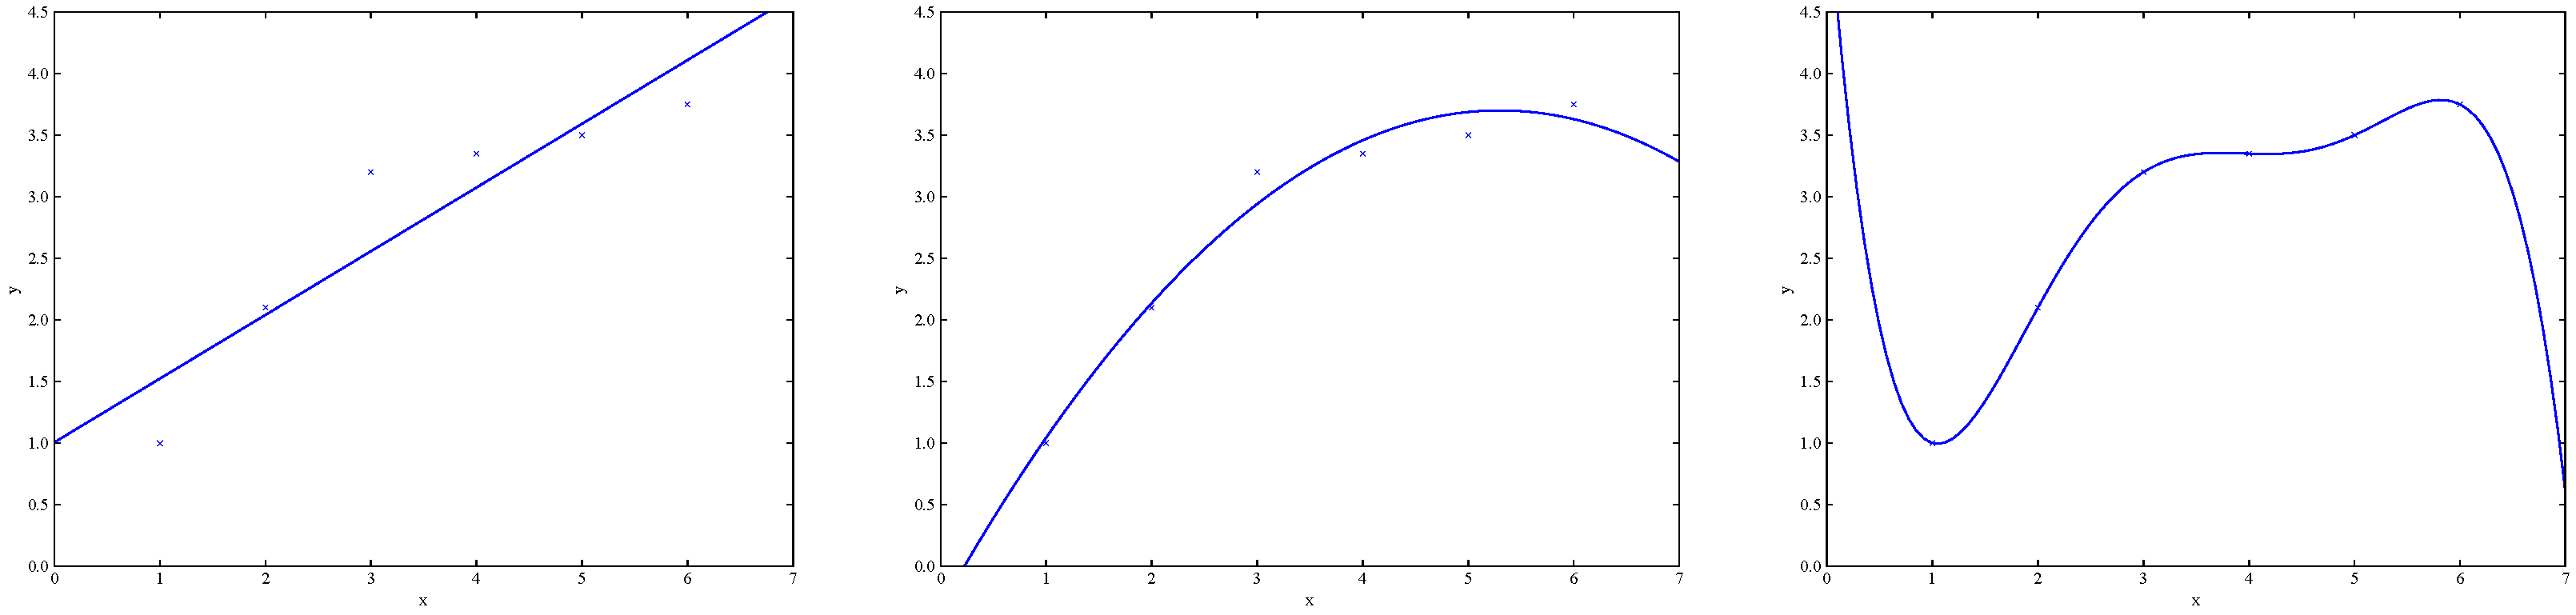
\includegraphics[width=0.93\linewidth]{figs/regression_plot.pdf}
\end{figure}

作为对比,如果我们添加一个额外的特征 $x^2$,然后拟合模型 $y = \theta_0 + \theta_1 x + \theta_2 x^2$,那么对数据的拟合效果可能会有所改善(参见中间图)。有人可能会简单地认为添加的特征越多越好。然而,过度添加特征也存在风险:最右边的图展示了拟合一个五阶多项式 $y = \sum_{j=0}^5 \theta_j x^j$ 的结果。尽管这条拟合曲线完美地穿过了所有数据点,我们也不能期望它能很好地预测不同居住区域 ($x$) 的房价 ($y$)。非正式地借用一下拟合的术语,可以说左边的图是\textbf{欠拟合 (underfitting)} 的一个例子——模型未能捕捉到数据中明显的结构——而右边的图则是一个\textbf{过拟合 (overfitting)} 的例子。(在课程后续的学习理论部分,我们将正式定义这些概念,并更严谨地探讨判断一个假设优劣的标准。)

正如先前讨论的,特征的选择对于确保学习算法的良好性能至关重要。(在后续关于模型选择的讨论中,我们也会介绍一些能够自动选择合适特征的算法。)在本节中,我们将简要介绍局部加权线性回归 (locally weighted linear regression, LWR) 算法。该算法假设有足够的训练数据,使得特征的选择不那么关键。鉴于读者将在作业中自行探索 LWR 算法的一些特性,本节的讲解将较为简略。

在原始的线性回归算法中,为了使用输入 $x$ 进行预测(即计算 $h(x)$ 的值),通常需要执行以下步骤:

\begin{enumerate}
    \item 拟合 $\theta$ 以最小化 $\sum_i (y^{(i)} - \theta^T x^{(i)})^2$。
    \item 输出 $\theta^T x$。
\end{enumerate}

相比之下,局部加权线性回归算法执行以下步骤:

\begin{enumerate}
    \item 拟合 $\theta$ 以最小化 $\sum_i w^{(i)} (y^{(i)} - \theta^T x^{(i)})^2$。
    \item 输出 $\theta^T x$。
\end{enumerate}

这里,$w^{(i)}$ 是非负的\textbf{权重 (weights)}。直观上,对于特定的训练样本 $i$,如果 $w^{(i)}$ 较大,则在确定参数 $\theta$ 时,模型会更倾向于使 $(y^{(i)} - \theta^T x^{(i)})^2$ 误差项尽可能小。反之,如果 $w^{(i)}$ 较小,则该误差项在拟合过程中基本上会被忽略。

一种常用的权重选择方法是\footnote{如果 $x$ 是向量,则推广为 $w^{(i)} = \exp(-(x^{(i)} - x)^T (x^{(i)} - x) / (2\tau^2))$,或者 $w^{(i)} = \exp(-(x^{(i)} - x)^T \Sigma^{-1} (x^{(i)} - x) / (2\tau^2))$,其中 $\tau$ 和 $\Sigma$ 需要选择合适的值。}
\[
    w^{(i)} = \exp\left(-\frac{(x^{(i)} - x)^2}{2\tau^2}\right).
\]
需要注意的是,权重取决于要评估的特定点 $x$。此外,如果 $|x^{(i)} - x|$ 的值很小,则 $w^{(i)}$ 接近 1;如果 $|x^{(i)} - x|$ 的值很大,则 $w^{(i)}$ 会很小。因此,在选择 $\theta$ 时,靠近查询点 $x$ 的训练样本(即其误差项 $y^{(i)} - \theta^T x^{(i)}$)会被赋予更高的“权重”。(另外需要说明的是,尽管权重的表达式形式上类似于高斯分布的概率密度函数,但 $w^{(i)}$ 与高斯分布并没有直接联系,特别是 $w^{(i)}$ 并非随机变量,无论是正态分布还是其他分布。)参数 $\tau$ 控制着训练样本的权重随其与查询点 $x$ 距离衰减的速度;$\tau$ 被称为\textbf{带宽 (bandwidth)} 参数,这也是在作业中需要进行实验的内容。

局部加权线性回归是我们遇到的第一个\textbf{非参数 (non-parametric)} 算法示例。之前讨论的(无权重)线性回归算法被称为\textbf{参数化 (parametric)} 学习算法,因为它通过固定数量的参数($\theta_i$)来拟合数据。一旦这些参数 $\theta_i$ 被确定并存储下来,就不再需要保留训练数据来进行后续的预测。相比之下,为了使用局部加权线性回归进行预测,必须保留整个训练集。术语“非参数”(大致)反映了这样一个事实:表示假设函数 $h$ 所需存储的数据量与训练集的大小呈线性关系。

\chapter{分类与逻辑回归}

现在我们转向分类问题。这与回归问题类似,主要区别在于需要预测的目标变量 $y$ 只能取有限的离散值。目前,我们将重点讨论二元分类 (binary classification) 问题,其中 $y$ 的取值仅限于 0 和 1。(这里讨论的大部分内容也适用于多类别分类情况。)例如,在构建垃圾邮件分类器时,$x^{(i)}$ 可以代表一封电子邮件的某些特征,而 $y$ 则表示该邮件是否为垃圾邮件(垃圾邮件为 1,非垃圾邮件为 0)。通常,0 被称为\textbf{负类 (negetive class)},1 被称为\textbf{正类 (positive class)},有时也用符号 “$-$” 和 “$+$” 表示。对于给定的输入特征 $x^{(i)}$,其对应的 $y^{(i)}$ 被称为该训练样本的\textbf{标签 (label)}。

\section{逻辑回归}\label{sec:2.1}

在处理分类问题时,我们可以暂时忽略目标变量 $y$ 是离散值这一特性,并沿用之前的线性回归算法来尝试预测给定输入 $x$ 的 $y$ 值。然而,很容易构造出这种方法表现极差的例子。直觉上,由于 $y$ 只能取 $\{0, 1\}$ 中的值,模型的输出 $h_\theta(x)$ 取大于 1 或小于 0 的值是没有意义的。为了解决这一问题,我们需要改变假设函数 $h_\theta(x)$ 的形式。具体而言,我们将选择:
\[
    h_\theta(x) = g(\theta^T x) = \frac{1}{1+e^{-\theta^T x}},
\]
其中
\[
    g(z) = \frac{1}{1+e^{-z}}.
\]
称为\textbf{逻辑函数 (logistic function)} 或 \textbf{S 形函数 (sigmoid function)}。下面是 $g(z)$ 的图像:

\begin{figure}[H]
    \centering
    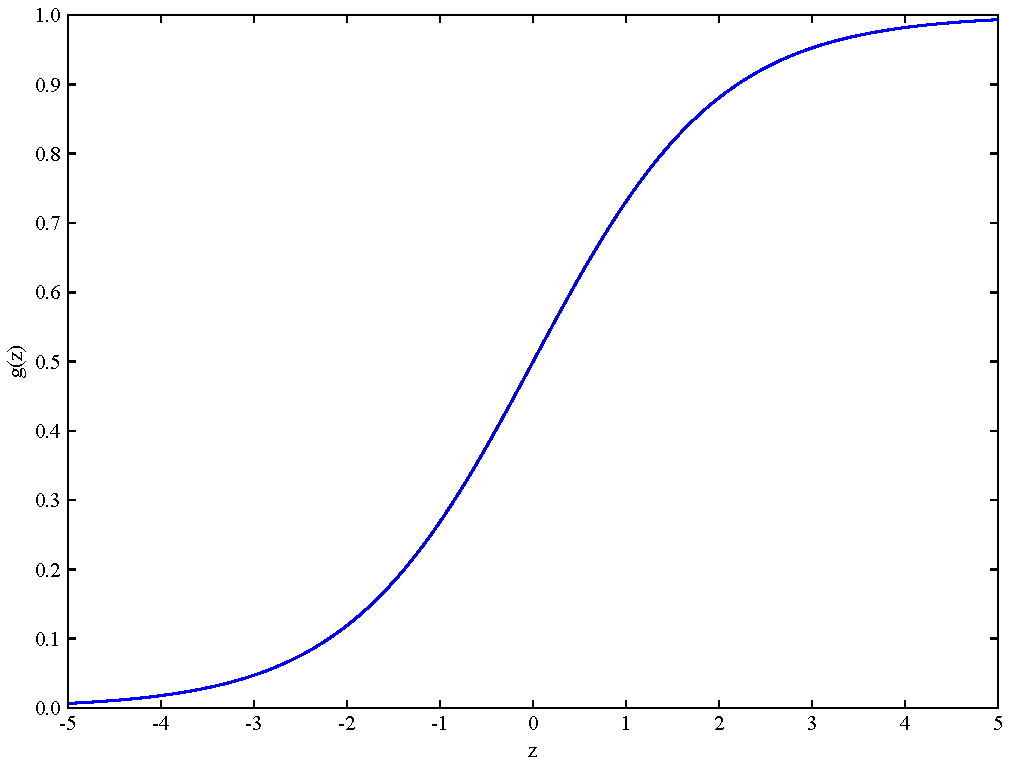
\includegraphics[width=0.5\linewidth]{figs/sigmoid.pdf}
    \label{fig:sigmoid}
\end{figure}

注意到 $g(z)$ 在 $z \to \infty$ 时趋于 1,在 $z \to -\infty$ 时趋于 0。此外,$g(z)$,因此 $h(x)$,始终介于 0 和 1 之间。和之前一样,这里约定 $x_0 = 1$,从而有 $\theta^T x = \theta_0 + \sum_{j=1}^d \theta_j x_j$。

现在先将 $g$ 的形式视为一个已知条件。其他从 0 平滑增加到 1 的函数也可以使用,但出于一些原因(稍后讨论广义线性模型(GLMs)和生成学习算法时会看到),选择 sigmoid 函数是相当自然的。在进一步展开之前,这里给出 sigmoid 函数导数的一个有用性质,记为 $g'$:
\[
    \begin{aligned}
        g'(z) &= \frac{d}{dz} \frac{1}{1+e^{-z}} \\ 
        &= \frac{1}{(1+e^{-z})^2} (e^{-z}) \\ 
        &= \frac{1}{1+e^{-z}} \cdot \left(1 - \frac{1}{1+e^{-z}}\right) \\ 
        &= g(z)(1 - g(z)).
    \end{aligned}
\]

那么,给定这样的逻辑回归模型,我们如何为其拟合 $\theta$ 呢?参照我们之前所见,最小二乘回归在一定假设下可以作为最大似然估计的一种形式。因此,我们也将为分类模型设定一组概率假设,然后通过最大似然估计的方式来拟合参数。

假设
\[
    \begin{aligned}
        P(y=1 \mid x; \theta) &= h_\theta(x) \\
        P(y=0 \mid x; \theta) &= 1 - h_\theta(x)
    \end{aligned}
\]
注意到上述两个概率表达式可以合并为一个更紧凑的形式
\[
    p(y \mid x; \theta) = (h_\theta(x))^y (1 - h_\theta(x))^{1-y}
\]
假设 $n$ 个训练样本是独立生成的,那么参数的似然可以写成
\[
    \begin{aligned}
        L(\theta) &= p(\vec{y} \mid X; \theta) \\ 
        &= \prod_{i=1}^n p(y^{(i)} \mid x^{(i)}; \theta) \\ 
        &= \prod_{i=1}^n (h_\theta(x^{(i)}))^{y^{(i)}} (1 - h_\theta(x^{(i)}))^{1-y^{(i)}}
    \end{aligned}
\]
和之前一样,最大化对数似然会更容易推导:
\begin{equation}
    \ell(\theta) = \log L(\theta) = \sum_{i=1}^n y^{(i)} \log h(x^{(i)}) + (1 - y^{(i)}) \log(1 - h(x^{(i)}))
    \label{eq:logistic_log_likelihood}
\end{equation}

那么,如何最大化这个似然函数呢呢?类似于线性回归的推导过程,我们可以采用梯度上升法。以向量形式表示,参数的更新规则为 $\theta := \theta + \alpha \nabla_\theta \ell(\theta)$。(注意更新公式中的正号,因为现在是在最大化函数,而不是最小化函数。)接下来,我们将从一个训练样本 $(x, y)$ 出发,推导随机梯度上升规则的导数:

\begin{align}
    \frac{\partial}{\partial \theta_j} \ell(\theta) &= \left(y \frac{1}{g(\theta^T x)} - (1-y) \frac{1}{1-g(\theta^T x)}\right) \frac{\partial}{\partial \theta_j} g(\theta^T x) \notag\\ 
    &= \left(y \frac{1}{g(\theta^T x)} - (1-y) \frac{1}{1-g(\theta^T x)}\right) g(\theta^T x)(1-g(\theta^T x)) \frac{\partial}{\partial \theta_j} \theta^T x \notag\\ 
    &= (y(1-g(\theta^T x)) - (1-y)g(\theta^T x)) x_j \notag\\
    &= (y - g(\theta^T x)) x_j \label{eq:partial_loss_theta}
\end{align}

上面的推导利用了 $g'(z) = g(z)(1-g(z))$ 这一点。这给出了随机梯度上升规则:
\[
    \theta_j := \theta_j + \alpha (y^{(i)} - h_\theta(x^{(i)})) x_j^{(i)}
\]
如果将推导出的逻辑回归更新规则与最小均方更新规则进行比较,会发现它们在形式上是相同的;但这并不是同一个算法,因为这里的 $h_\theta(x^{(i)})$ 是 $\theta^T x^{(i)}$ 的非线性函数。尽管如此,对于一个截然不同的算法和学习问题,却得到了相同的更新规则,这确实有些令人惊讶。这仅仅是巧合吗?抑或是背后存在更深层的原因?我们将在讨论广义线性模型(GLM)时解答这个问题。

\begin{remark}\label{remark:2.1.1}
    同一个损失函数的另一种表示方式也很有用,特别是在第 \ref{sec:7.1} 节研究非线性模型时。
\end{remark}
\noindent 设逻辑损失函数 $\ell_{\text{logistic}}: \mathbb{R} \times \{0, 1\} \to \mathbb{R}_{\ge 0}$ 定义为
\begin{equation}
    \ell_{\text{logistic}}(t, y) \triangleq y \log(1 + \exp(-t)) + (1 - y) \log(1 + \exp(t)).
\end{equation}
通过代入 $h_\theta(x) = 1/(1 + e^{-\theta^T x})$,可以验证负对数似然(方程 \eqref{eq:logistic_log_likelihood} 中 $\ell(\theta)$ 的负值)可以改写为
\begin{equation}
    -\ell(\theta) = \ell_{\text{logistic}}(\theta^T x, y).
\end{equation}
通常 $\theta^T x$ 或 $t$ 称为 \textit{logit}。稍作运算可得
\begin{align}
    \frac{\partial \ell_{\text{logistic}}(t, y)}{\partial t} &= y \frac{-\exp(-t)}{1 + \exp(-t)} + (1 - y) \frac{1}{1 + \exp(-t)} \\ 
    &= \frac{1}{1 + \exp(-t)} - y. \label{eq:2.6}
\end{align}
然后,使用链式法则,得到
\begin{align}
    \frac{\partial}{\partial \theta_j} \ell(\theta) &= - \frac{\partial \ell_{\text{logistic}}(t, y)}{\partial t} \cdot \frac{\partial t}{\partial \theta_j} \\ 
    &= (y-1/(1+\exp(-t))) \cdot x_j = (y - h_\theta(x)) x_j, 
\end{align}
这与方程 \eqref{eq:partial_loss_theta} 的推导是一致的。在第 \ref{sec:7.1} 节中,会看到这种观点可以扩展到非线性模型。

\section{离题:感知器学习算法}

现在,我们将简要讨论一个具有历史意义的算法,该算法在后续讨论学习理论时也将再次被提及。考虑对逻辑回归方法进行修改,“强制”其输出值为 0 或 1。为此,一个自然而然的想法是将函数 $g$ 的定义改为阈值函数:
\[
    g(z) = 
    \begin{cases} 
        1 & \text{若 } z \ge 0 \\
        0 & \text{若 } z < 0 
    \end{cases}
\]
如果像之前一样令 $h_\theta(x) = g(\theta^T x)$,但使用上述修改后的 $g$ 定义,并且使用更新规则
\[
    \theta_j := \theta_j + \alpha (y^{(i)} - h_\theta(x^{(i)})) x_j^{(i)}.
\]
那么就得到了\textbf{感知机学习算法 (perceptron learning algorithm)}。

在 20 世纪 60 年代,有人认为“感知机”是脑中单个神经元如何工作的一个粗略模型。考虑到该算法的简单性,在讨论学习理论时,它也将为分析提供一个起点。然而,请注意,尽管感知机看起来与其他讨论过的算法相似,但它实际上与逻辑回归和最小二乘线性回归是完全不同类型的算法;特别是,很难从概率角度解释感知机的预测结果,或者将感知机推导为最大似然估计算法。


\section{多类别分类}\label{sec:2.3}

考虑一个分类问题,其中响应变量 $y$ 可以取 $k$ 个值中的任意一个,即 $y \in \{1, 2, \dots, k\}$。例如,除了将电子邮件分为垃圾邮件或非垃圾邮件这两类(这是一个二元分类问题),也可能希望将其分为三类,例如垃圾邮件、个人邮件和工作相关邮件。标签/响应变量仍然是离散的,但现在可以取超过两个值。因此,将它建模为服从多项分布。

在这种情况下,$p(y \mid x; \theta)$ 是关于 $k$ 个可能的离散结果的分布,因此是多项分布。回想一下,多项分布涉及 $k$ 个数 $\phi_1, \dots, \phi_k$,它们指定了每个结果的概率。注意,这些数必须满足 $\sum_{i=1}^k \phi_i = 1$。将设计一个参数化模型,该模型输出满足此约束的 $\phi_1, \dots, \phi_k$,给定输入 $x$。

引入 $k$ 组参数 $\theta_1, \dots, \theta_k$,每组参数都是 $\mathbb{R}^d$ 中的一个向量。直观地,希望使用 $\theta_1^T x, \dots, \theta_k^T x$ 来表示$\phi_1, \dots, \phi_k$,即概率 $P(y = 1 \mid x; \theta), \dots, P(y = k \mid x; \theta)$。然而,这种直接方法存在两个问题。首先,$\theta_j^T x$ 不一定在 $[0, 1]$ 范围内。其次,$\theta_j^T x$ 的总和不一定为 1。因此,将使用 softmax 函数将 $(\theta_1^T x, \dots, \theta_k^T x)$ 转换为一个非负且总和为 1 的概率向量。

定义函数 $\text{softmax}: \mathbb{R}^k \to \mathbb{R}^k$ 如下:
\begin{equation}
    \text{softmax}(t_1, \dots, t_k) = 
    \begin{bmatrix} 
        \frac{\exp(t_1)}{\sum_{j=1}^k \exp(t_j)} \\
        \vdots \\
        \frac{\exp(t_k)}{\sum_{j=1}^k \exp(t_j)}
    \end{bmatrix}.
\end{equation}
softmax 函数的输入,即这里的向量 $t$,通常被称为 \textit{logits}。注意,根据定义,softmax 函数的输出始终是一个概率向量,其分量非负且总和为 1。

令 $(t_1, \dots, t_k) = (\theta_1^T x, \dots, \theta_k^T x)$。将 softmax 函数应用于 $(t_1, \dots, t_k)$,并将输出用作概率 $P(y = 1 \mid x; \theta), \dots, P(y = k \mid x; \theta)$。得到以下概率模型:
\begin{equation}
    \begin{bmatrix} 
        P(y = 1 \mid x; \theta) \\
        \vdots& \\
        P(y = k \mid x; \theta)
    \end{bmatrix} =
    \text{softmax}(t_1, \dots, t_k) = 
    \begin{bmatrix} 
    &\frac{\exp(\theta_1^T x)}{\sum_{j=1}^k \exp(\theta_j^T x)}& \\
    &\vdots& \\
    &\frac{\exp(\theta_k^T x)}{\sum_{j=1}^k \exp(\theta_j^T x)}&
    \end{bmatrix}.
\end{equation}
为了符号上的方便,令 $\phi_i = \frac{\exp(t_i)}{\sum_{j=1}^k \exp(t_j)}$。更简洁地,上面的方程可以写成:
\begin{equation}
    P(y = i \mid x; \theta) = \phi_i = \frac{\exp(t_i)}{\sum_{j=1}^k \exp(t_j)} = \frac{\exp(\theta_i^T x)}{\sum_{j=1}^k \exp(\theta_j^T x)}.
\end{equation}
接下来,计算单个样本 $(x, y)$ 的负对数似然。
\begin{equation}
    -\log p(y \mid x, \theta) = -\log\left(\frac{\exp(t_y)}{\sum_{j=1}^k \exp(t_j)}\right) = -\log\left(\frac{\exp(\theta_y^T x)}{\sum_{j=1}^k \exp(\theta_j^T x)}\right).
\end{equation}
因此,损失函数,即训练数据的负对数似然,由下式给出:
\begin{equation}
    \ell(\theta) = \sum_{i=1}^n -\log\left(\frac{\exp(\theta_{y^{(i)}}^T x^{(i)})}{\sum_{j=1}^k \exp(\theta_j^T x^{(i)})}\right).
    \label{eq:multiclass_loss}
\end{equation}
定义交叉熵损失 $\ell_{\text{ce}}: \mathbb{R}^k \times \{1, \dots, k\} \to \mathbb{R}_{\ge 0}$ 是很方便的,它将上述复杂的方程模块化为\footnote{这里命名存在一些歧义。有些人将交叉熵损失定义为将概率向量(在本讲义中用 $\phi$ 表示)和标签 $y$ 映射到实数的函数,并将本讲义中的交叉熵损失称为 softmax-交叉熵损失。本讲义选择当前的命名约定是因为它与大多数现代深度学习库(如 PyTorch 和 Jax)的命名一致。}:
\begin{equation}
    \ell_{\text{ce}}((t_1, \dots, t_k), y) = -\log \left( \frac{\exp(t_y)}{\sum_{j=1}^k \exp(t_j)} \right).
\end{equation}
使用此记号,方程 \eqref{eq:multiclass_loss} 可以简写为:
\begin{equation}
    \ell(\theta) = \sum_{i=1}^n \ell_{\text{ce}}((\theta_1^\top x^{(i)}, \dots, \theta_k^\top x^{(i)}), y^{(i)}).
\end{equation}
此外,交叉熵损失的梯度也很便于推导。令 $t = (t_1, \dots, t_k)$,并回顾 $\phi_i = \frac{\exp(t_i)}{\sum_{j=1}^k \exp(t_j)}$。可以推导出:
\begin{equation}
    \frac{\partial \ell_{\text{ce}}(t, y)}{\partial t_i} = \phi_i - {1}\{y=i\},
\end{equation}
其中 ${1}\{\cdot\}$ 是指示函数,即当 $y=i$ 时 ${1}\{y=i\} = 1$,当 $y \ne i$ 时 $\{y=i\} = 0$。向量化形式如下,这对于第 \ref{chapter:7} 章将很有用:
\begin{equation}
    \frac{\partial \ell_{\text{ce}}(t, y)}{\partial t} = \phi - e_y,\label{eq:2.17}
\end{equation}
其中 $e_s \in \mathbb{R}^k$ 是第 $s$ 个标准基向量(其中第 $s$ 个分量是 1,其余所有分量都是零)。使用链式法则,有:
\begin{equation}
    \frac{\partial \ell_{\text{ce}}((\theta_1^\top x, \dots, \theta_k^\top x), y)}{\partial \theta_i} = \frac{\partial \ell(t, y)}{\partial t_i} \frac{\partial t_i}{\partial \theta_i} = (\phi_i - {1}\{y=i\}) \cdot x.
\end{equation}
因此,损失函数关于参数 $\theta_i$ 的梯度为:
\begin{equation}
    \frac{\partial \ell(\theta)}{\partial \theta_i} = \sum_{j=1}^n (\phi_i^{(j)} - {1}\{y^{(j)}=i\}) \cdot x^{(j)},
\end{equation}
其中 $\phi_i^{(j)} = \frac{\exp(\theta_i^\top x^{(j)})}{\sum_{s=1}^k \exp(\theta_s^\top x^{(j)})}$ 是模型预测样本 $x^{(j)}$ 属于类别 $i$ 的概率。利用上述梯度,可以使用(随机)梯度下降来最小化损失函数 $\ell(\theta)$。

\section{最大化 \texorpdfstring{$\ell(\theta)$}{l(theta)} 的另一种算法}

回到以 sigmoid 为 $g(z)$ 函数的逻辑回归,现在讨论一种不同的最大化 $\ell(\theta)$ 的算法。

首先,考虑牛顿法用于寻找函数零点。具体来说,假设有一个函数 $f: \mathbb{R} \to \mathbb{R}$,并且希望找到一个 $\theta$ 值使得 $f(\theta) = 0$。这里 $\theta \in \mathbb{R}$ 是一个实数。牛顿法执行以下更新:
\[
    \theta := \theta - \frac{f(\theta)}{f'(\theta)}.
\]
这种方法有一种自然的解释:将函数 $f$ 通过其在当前猜测值 $\theta$ 处的切线进行近似,然后求解该切线等于零的点,并将该点作为 $\theta$ 的下一个猜测值。

以下是牛顿法实际应用的图示:

\begin{figure}[H]
  \centering
  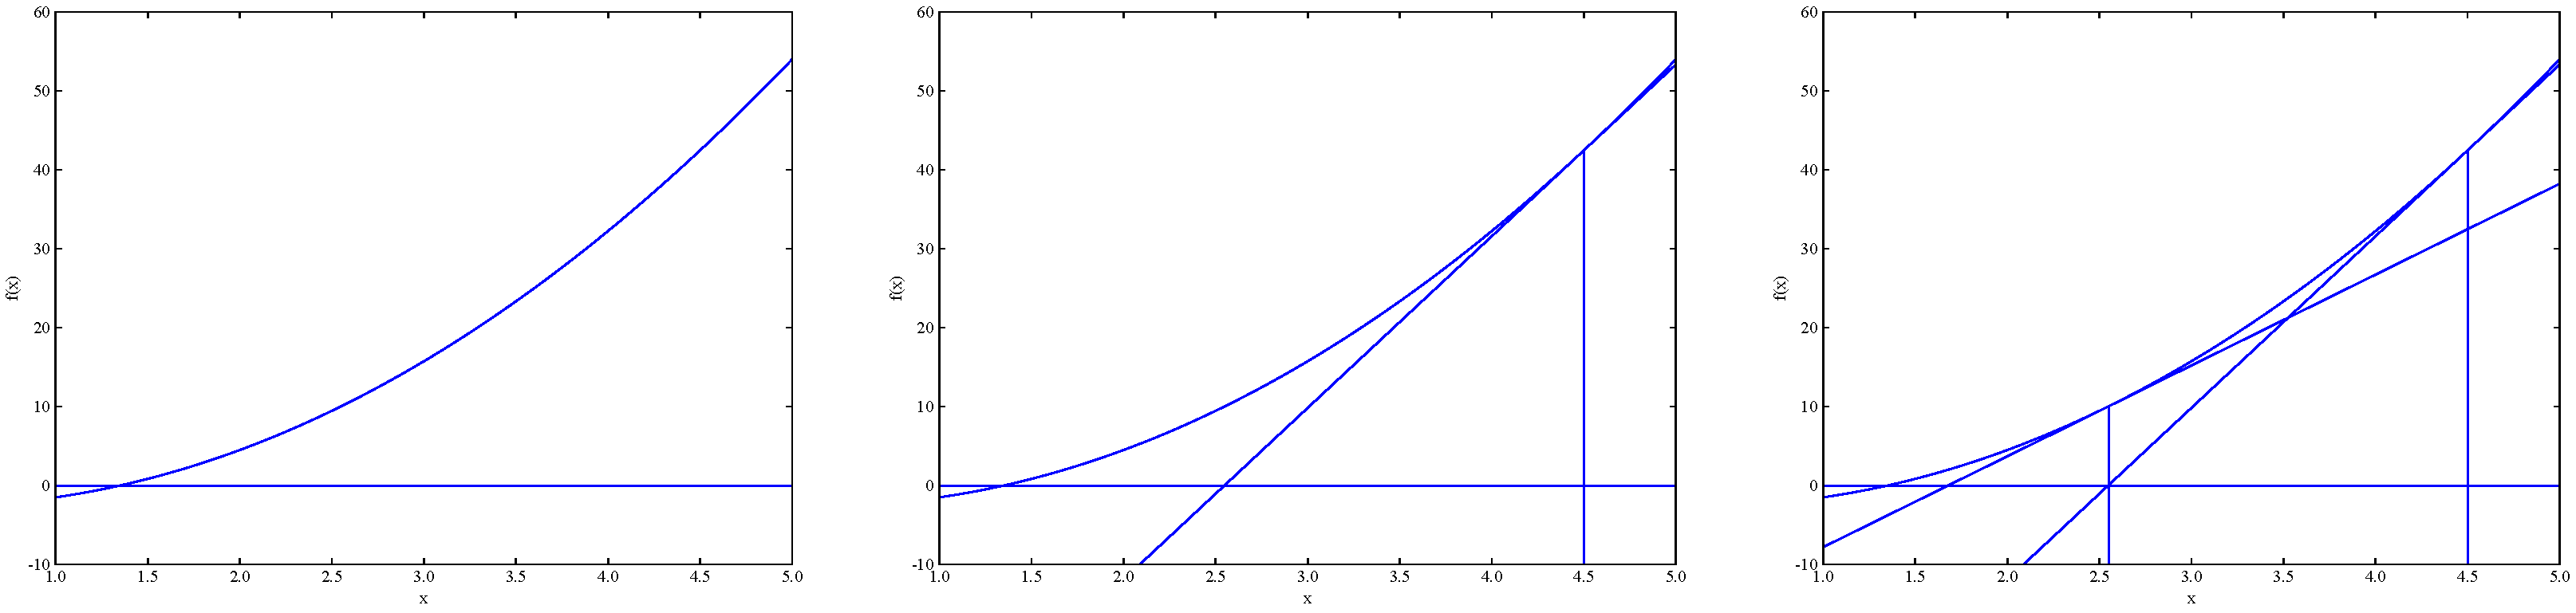
\includegraphics[width=0.93\linewidth]{figs/newton_iteration.pdf}
\end{figure}

\setcounter{footnote}{0}
\renewcommand{\thefootnote}{\fnsymbol{footnote}}
在最左边的图中,可以看到函数 $f$ 与直线 $y=0$。尝试找到一个 $\theta$ 使得 $f(\theta)=0$;实现这一点的 $\theta$ 值大约是 1.3。假设初始化的算法的 $\theta$ 值为 4.5。然后牛顿法拟合一条在 $\theta=4.5$ 处与 $f$ 相切的直线,并求解该直线等于 0 的点(中间图)。这给出了 $\theta$ 的下一个猜测值,大约是 2.6。最右边的图显示了再进行一次迭代的结果,更新后的 $\theta$ 大约是 1.6。再经过几次迭代后,将迅速接近 $\theta = 1.3$\footnote{译者注:由于不知道原书所用函数的解析形式,这里译者画的图与原图稍有偏差,$\theta$的猜测值也稍有变化。}。
\setcounter{footnote}{1}
\renewcommand{\thefootnote}{\arabic{footnote}}

牛顿法提供了一种求解 $f(\theta)=0$ 的方法。如果希望最大化某个函数 $\ell$ 呢? $\ell$ 的最大值对应于其一阶导数 $\ell'(\theta)$ 为零的点。因此,令 $f(\theta) = \ell'(\theta)$,可以使用相同的算法来最大化 $\ell$,并得到更新规则:
\[
    \theta := \theta - \frac{\ell'(\theta)}{\ell''(\theta)}.
\]
(思考题:如果希望使用牛顿法来最小化而不是最大化一个函数,这会如何改变?)

最后,在逻辑回归中,$\theta$ 是向量,因此需要将牛顿法推广到此情况。牛顿法在此多维设置中的推广(也称为牛顿-拉普森法)由下式给出
\[
    \theta := \theta - H^{-1} \nabla_\theta \ell(\theta).
\]
这里,$\nabla_\theta \ell(\theta)$ 是 $\ell(\theta)$ 对 $\theta_i$ 的偏导数向量,而 $H$ 是一个 $d \times d$ 矩阵(实际上,如果包含截距项,则是 $(d+1) \times (d+1)$ 矩阵),称为\textbf{Hessian} 矩阵,其元素由下式给出
\[
    H_{ij} = \frac{\partial^2 \ell(\theta)}{\partial \theta_i \partial \theta_j}.
\]
牛顿法通常比(批量)梯度下降收敛更快,并且需要更少的迭代次数即可非常接近最小值。然而,牛顿法迭代一次比梯度下降迭代一次更昂贵,因为它需要找到一个 $d \times d$ 的 Hessian 矩阵并求逆;但只要 $d$ 不太大,通常总体上会快得多。当牛顿法应用于最大化逻辑回归对数似然函数 $\ell(\theta)$ 时,所得方法也称为 \textbf{Fisher scoring}。

\chapter{广义线性模型}
到目前为止,我们已经讨论了一个回归示例和一个分类示例。在回归示例中,有 $y|x; \theta \sim \mathcal{N}(\mu, \sigma^2)$,在分类示例中,有 $y|x; \theta \sim \text{Bernoulli}(\phi)$,其中 $\mu$ 和 $\phi$ 是 $x$ 和 $\theta$ 的函数。在本节中,将展示这两种方法都是更广泛的模型族——称为广义线性模型(GLMs)\footnote{本节材料受到 Michael I. Jordan 的 \textit{Learning in graphical models}(未出版的书稿)以及 McCullagh 和 Nelder 的 \textit{Generalized Linear Models (2nd ed.)} 的启发。}——的特例。我们还将展示广义线性模型族中的其他模型如何推导并应用于其他分类和回归问题。

\section{指数族}

为了逐步了解广义线性模型,首先定义指数族分布。如果一类分布可以写成以下形式,则称其为指数族:
\begin{equation}
    p(y; \eta) = b(y) \exp(\eta^T T(y) - a(\eta))
    \label{eq:exp_family}
\end{equation}
这里,$\eta$ 称为\textbf{自然参数 (natural parameter)}(也称为\textbf{典范参数 (canonical parameter)});$T(y)$ 是\textbf{充分统计量 (sufficient statistic)}(对于所考虑的分布,通常有 $T(y)=y$);而 $a(\eta)$ 是\textbf{对数配分函数 (log partition function)}。量 $e^{-a(\eta)}$ 实际上起着归一化常数的作用,确保分布 $p(y; \eta)$ 在 $y$ 上的和或积分等于 1。

固定的 $T$, $a$ 和 $b$ 定义了一个由 $\eta$ 参数化的\textit{族 (family)}(或分布集);随着 $\eta$ 的变化,将得到该族中的不同分布。

现在展示伯努利分布和高斯分布是指数族分布的示例。具有均值 $\phi$ 的伯努利分布,记为 $\text{Bernoulli}(\phi)$,指定了在 $y \in \{0, 1\}$ 上的分布,使得 $p(y=1; \phi) = \phi$;$p(y=0; \phi) = 1-\phi$。随着 $\phi$ 的变化,可以得到具有不同均值的伯努利分布。现在我们推导改变 $\phi$ 得到的这些伯努利分布属于指数族;也就是说,存在一种 $T, a, b$ 的选择,使得公式 \eqref{eq:exp_family} 恰好成为伯努利分布。

将伯努利分布写为:
\[
\begin{aligned}
    p(y; \phi) &= \phi^y (1-\phi)^{1-y} \\
    &= \exp\left(y \log \phi + (1-y) \log(1-\phi)\right) \\
    &= \exp\left(\left(\log\left(\frac{\phi}{1-\phi}\right)\right)y + \log(1-\phi)\right).
\end{aligned}
\]
因此,自然参数由 $\eta = \log(\phi/(1-\phi))$ 给出。有趣的是,如果通过求解 $\phi$ 关于 $\eta$ 的表达式来反转这个定义,得到 $\phi = 1/(1+e^{-\eta})$。这是熟悉的 sigmoid 函数!在将逻辑回归推导为广义线性模型时,这将再次出现。为了完成伯努利分布作为指数族分布的形式化,还需要以下各项:
\[
\begin{aligned}
    T(y) &= y \\
    a(\eta) &= -\log(1-\phi) \\
    &= \log(1+e^\eta) \\
    b(y) &= 1
\end{aligned}
\]
这表明伯努利分布可以通过选择适当的 $T, a, b$ 从而写成公式 \eqref{eq:exp_family} 的形式。

接下来考虑高斯分布。回想一下,在线性回归推导中,$\sigma^2$ 的值对最终选择的 $\theta$ 和 $h_\theta(x)$ 没有影响。因此,可以在不改变任何内容的情况下选择任意的 $\sigma^2$ 值。为了简化下面的推导,令 $\sigma^2 = 1$。\footnote{如果将 $\sigma^2$ 作为一个变量,高斯分布也可以显示为指数族,其中 $\eta \in \mathbb{R}^2$ 现在是一个二维向量,它取决于 $\mu$ 和 $\sigma$。然而,出于广义线性模型的目的,$\sigma^2$ 参数也可以通过考虑指数族的一个更一般的定义来处理:$p(y; \eta, \tau) = b(a, \tau) \exp((\eta^T T(y) - a(\eta))/c(\tau))$。这里,$\tau$ 称为\textbf{散布参数 (dispersion parameter)},对于 高斯分布,$c(\tau) = \sigma^2$;但考虑到上面的简化,这里不需要更一般的定义。}有:
\[
\begin{aligned}
    p(y; \mu) &= \frac{1}{\sqrt{2\pi}} \exp\left(-\frac{1}{2}(y-\mu)^2\right) \\
    &= \frac{1}{\sqrt{2\pi}} \exp\left(-\frac{1}{2}y^2 + \mu y - \frac{1}{2}\mu^2\right) \\
    &= \frac{1}{\sqrt{2\pi}} \exp\left(-\frac{1}{2}y^2\right) \cdot \exp\left(\mu y - \frac{1}{2}\mu^2\right).
\end{aligned}
\]
因此, 高斯分布属于指数族,其中
\[
\begin{aligned}
    \eta &= \mu \\
    T(y) &= y \\
    a(\eta) &= \mu^2/2 \\
    &= \eta^2/2 \\
    b(y) &= (1/\sqrt{2\pi})\exp(-y^2/2).
\end{aligned}
\]

还有许多其他分布也属于指数族:多项分布(稍后将看到)、泊松分布(用于建模计数数据;另请参阅问题集)、伽马分布和指数分布(用于建模连续非负随机变量,例如时间间隔)、Beta 分布和 Dirichlet 分布(用于概率分布)等等。在下一节中,将描述构建模型的一般“配方”,其中 $y$(给定 $x$ 和 $\theta$)来自于这些分布中的任何一个。


\section{构造广义线性模型}

假设希望构建一个模型来估计在给定小时内到达商店的顾客数量(或网站的页面浏览量 $y$),基于某些特征 $x$,例如商店促销、近期广告、天气、星期几等等。已知泊松分布通常能很好地模拟访客数量。知道了这一点,如何为问题构建模型?幸运的是,泊松分布是指数族分布,因此可以应用广义线性模型。在本节中,将描述一种构建用于解决此类问题的广义线性模型的方法。

更一般地,考虑一个分类或回归问题,希望预测某个随机变量 $y$ 作为 $x$ 的函数的值。为了推导针对此问题的广义线性模型,将对给定 $x$ 的 $y$ 的条件分布和模型做出以下三个假设:

\begin{enumerate}
    \item $y|x; \theta \sim \text{ExponentialFamily}(\eta)$。也就是说,给定 $x$ 和 $\theta$, $y$ 的分布遵循参数为 $\eta$ 的某个指数族分布;
    \item 给定 $x$,目标是预测 $T(y)$ 的期望值。在大多数示例中,$T(y)=y$,因此这意味着希望学习到的假设 $h$ 的输出预测 $h(x)$ 满足 $h(x) = E[y|x]$。(注意,这个假设在逻辑回归和线性回归中对于 $h_\theta(x)$ 的选择是满足的。例如,在逻辑回归中,$h_\theta(x) = p(y=1|x; \theta) = 0 \cdot p(y=0|x; \theta) + 1 \cdot p(y=1|x; \theta) = E[y|x; \theta]$.);
    \item 自然参数 $\eta$ 和输入 $x$ 线性相关:$\eta = \theta^T x$。(或者,如果 $\eta$ 是向量值,则 $\eta_i = \theta_i^T x$.)
\end{enumerate}

第三个假设可能看起来最不合理,最好将其视为设计广义线性模型的“设计选择”,而不是一个固有的假设。这三个假设/设计选择将允许推导出非常优雅的一类学习算法,即广义线性模型,它们具有许多理想的特性,例如易于学习。此外,由此产生的模型对于建模不同类型的 $y$ 分布非常有效;例如,很快将展示逻辑回归和普通最小二乘都可以作为广义线性模型推导出来。

\subsection{普通最小二乘}

为了展示普通最小二乘是广义线性模型族的一个特例,考虑目标变量 $y$(在广义线性模型术语中也称为\textbf{响应变量 (response variable)})是连续的情况,并将给定 $x$ 的 $y$ 的条件分布建模为高斯分布 $N(\mu, \sigma^2)$。(这里,$\mu$ 可能取决于 $x$.)因此,令上面的 $\text{ExponentialFamily}(\eta)$ 分布为 高斯分布。如前所述,在将高斯分布公式化为指数族分布时,有 $\mu = \eta$。因此,有
\[
\begin{aligned}
    h_\theta(x) &= E[y|x; \theta] \\
    &= \mu \\
    &= \eta \\
    &= \theta^T x.
\end{aligned}
\]
第一个等号来自于上面的假设 2;第二个等号来自于 $y|x; \theta \sim N(\mu, \sigma^2)$,因此其期望值由 $\mu$ 给出;第三个等号来自于假设 1(以及之前推导中表明在将高斯分布公式化为指数族分布时 $\mu = \eta$);最后一个等号来自于假设 3。

\subsection{逻辑回归}

现在考虑逻辑回归。这里感兴趣的是二分类问题,因此 $y \in \{0, 1\}$。鉴于 $y$ 是二值变量,选择伯努利分布族来建模给定 $x$ 的 $y$ 的条件分布是很自然的。在将伯努利分布公式化为指数族分布时,有 $\phi = 1/(1 + e^{-\eta})$。此外,注意如果 $y|x; \theta \sim \text{Bernoulli}(\phi)$,则 $E[y|x; \theta] = \phi$。因此,按照与普通最小二乘类似的推导,得到:
\[
\begin{aligned}
    h_\theta(x) &= E[y|x; \theta] \\
    &= \phi \\
    &= 1/(1 + e^{-\eta}) \\
    &= 1/(1 + e^{-\theta^T x})
\end{aligned}
\]
因此,这给出了形式为 $h_\theta(x) = 1/(1 + e^{-\theta^T x})$ 的假设函数。如果之前曾想知道如何得到逻辑函数 $1/(1 + e^{-z})$ 的形式,这就是一个答案:一旦假设给定 $x$ 的 $y$ 服从伯努利分布,它就作为广义线性模型和指数族分布定义的必然结果出现了。

这里引入一些额外的术语,将自然参数映射到分布均值的函数 $g$($g(\eta) = E[T(y); \eta]$),称为\textbf{典范响应函数 (canonical response1 function)}。其逆函数 $g^{-1}$ 称为\textbf{典范连接函数 (canonical link function)}。因此,高斯族分布的典范响应函数就是恒等函数;伯努利分布的典范响应函数是逻辑函数\footnote{许多文献使用 $g$ 表示连接函数,$g^{-1}$ 表示响应函数;但这里使用的符号继承自早期的机器学习文献,将与课程其余部分使用的符号更一致。}。

\chapter{生成式学习算法}

到目前为止,我们讨论的主要是学习这样的一类算法,这些算法建模给定 $x$ 的情况下 $y$ 的条件分布 $p(y|x; \theta)$。例如,逻辑回归将 $p(y|x; \theta)$ 建模为 $h_\theta(x) = g(\theta^T x)$,其中 $g$ 是 sigmoid 函数。在本章中,将讨论一种不同类型的学习算法。

考虑一个分类问题,其中希望根据动物的一些特征来区分大象 ($y=1$) 和狗 ($y=0$)。给定一个训练集,像逻辑回归或感知机算法(本质上)试图找到一条直线——也就是一个决策边界——来分隔大象和狗。然后,为了将新动物分类为大象或狗,检查其落在决策边界的哪一侧,并据此做出预测。

这里介绍一种不同的方法。首先,观察大象,可以建立一个关于大象外观的模型。然后,观察狗,可以建立一个关于狗外观的独立模型。最后,为了对新动物进行分类,可以将新动物与大象模型进行匹配,并将其与狗模型进行匹配,以查看新动物是否更像在训练集中看到的大象或狗。

试图直接学习 $p(y|x)$ 的算法(如逻辑回归),或试图直接学习从输入空间 $\mathcal{X}$ 到标签 $\{0, 1\}$ 的映射的算法(如感知机算法)称为\textbf{判别式 (discriminative)} 学习算法。这里,将讨论那些试图建模 $p(x|y)$(和 $p(y)$)的算法。这些算法称为\textbf{生成式 (generative)} 学习算法。例如,如果 $y$ 表示一个样本是狗 ($0$) 还是大象 ($1$),则 $p(x|y=0)$ 建模狗的特征分布,$p(x|y=1)$ 建模大象的特征分布。

在建模 $p(y)$(称为\textbf{类先验 (class priors)})和 $p(x|y)$ 之后,算法可以利用贝叶斯定理推导出给定 $x$ 时 $y$ 的后验分布:
\[
    p(y|x) = \frac{p(x|y)p(y)}{p(x)}.
\]
这里,分母由 $p(x) = p(x|y=1)p(y=1) + p(x|y=0)p(y=0)$ 给出(根据概率的标准性质,可以验证这一点),因此也可以用学到的 $p(x|y)$ 和 $p(y)$ 来表示。实际上,如果计算 $p(y|x)$ 是为了进行预测,那么并不需要计算分母,因为
\[
\begin{aligned}
    \arg \max_y p(y|x) &= \arg \max_y \frac{p(x|y)p(y)}{p(x)} \\
    &= \arg \max_y p(x|y)p(y).
\end{aligned}
\]

\section{高斯判别分析}

将要介绍的第一个生成式学习算法是高斯判别分析 (GDA)。在这个模型中,假设 $p(x|y)$ 服从多元正态分布。在介绍 GDA 模型本身之前,先简要讨论一下多元正态分布的性质。

\subsection{多元正态分布}

$d$ 维的多元正态分布,也称为多元高斯分布,由\textbf{均值向量 (mean vector)} $\mu \in \mathbb{R}^d$ 和\textbf{协方差矩阵 (covariance matrix)} $\Sigma \in \mathbb{R}^{d \times d}$ 参数化,其中 $\Sigma \ge 0$ 是对称正半定矩阵。其密度函数写为 $\mathcal{N}(\mu, \Sigma)$,形式如下:
\[
    p(x; \mu, \Sigma) = \frac{1}{(2\pi)^{d/2}|\Sigma|^{1/2}} \exp\left(-\frac{1}{2}(x-\mu)^T \Sigma^{-1}(x-\mu)\right).
\]
在上面的方程中,$|\Sigma|$ 表示矩阵 $\Sigma$ 的行列式。
对于服从 $\mathcal{N}(\mu, \Sigma)$ 分布的随机变量 $X$,其均值(毫不意外地)由 $\mu$ 给出:
\[
    \mathrm{E}[X] = \int_x x p(x; \mu, \Sigma) dx = \mu
\]
向量值随机变量 $Z$ 的\textbf{协方差}定义为 $\text{Cov}(Z) = \mathrm{E}[(Z - \mathrm{E}[Z])(Z - \mathrm{E}[Z])^T]$。这推广了实值随机变量的方差概念。协方差也可以定义为 $\text{Cov}(Z) = \mathrm{E}[ZZ^T] - (\mathrm{E}[Z])(\mathrm{E}[Z])^T$。(可以自行证明这两个定义是等价的。)如果 $X \sim \mathcal{N}(\mu, \Sigma)$,则
\[
    \mathrm{Cov}(X) = \Sigma.
\]

以下是一些高斯分布密度函数的示例:

\begin{figure}[H]
    \centering
    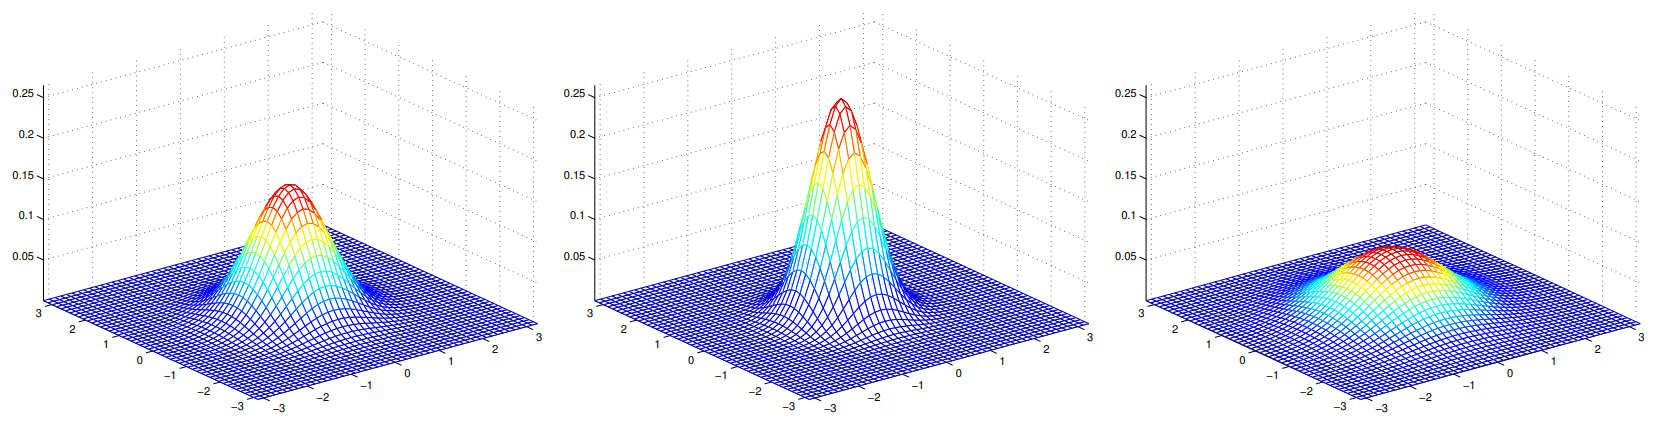
\includegraphics[width=1.0\linewidth]{figs/gaussian_density1.png}
\end{figure}

最左边的图显示的是均值为零(即 $2 \times 1$ 零向量)、协方差矩阵为 $\Sigma = I$(即 $2 \times 2$ 单位矩阵)的高斯分布。均值为零、协方差为单位矩阵的高斯分布也称为\textbf{标准正态分布}。中间的图显示的是均值为零、$\Sigma = 0.6I$ 的高斯分布的密度;最右边的图显示的是 $\Sigma = 2I$ 的高斯分布的密度。可以看到,随着 $\Sigma$ 变大,高斯分布变得更加“分散”,而随着 $\Sigma$ 变小,分布变得更加“紧凑”。

接下来看一些更多的例子。

\begin{figure}[H]
    \centering
    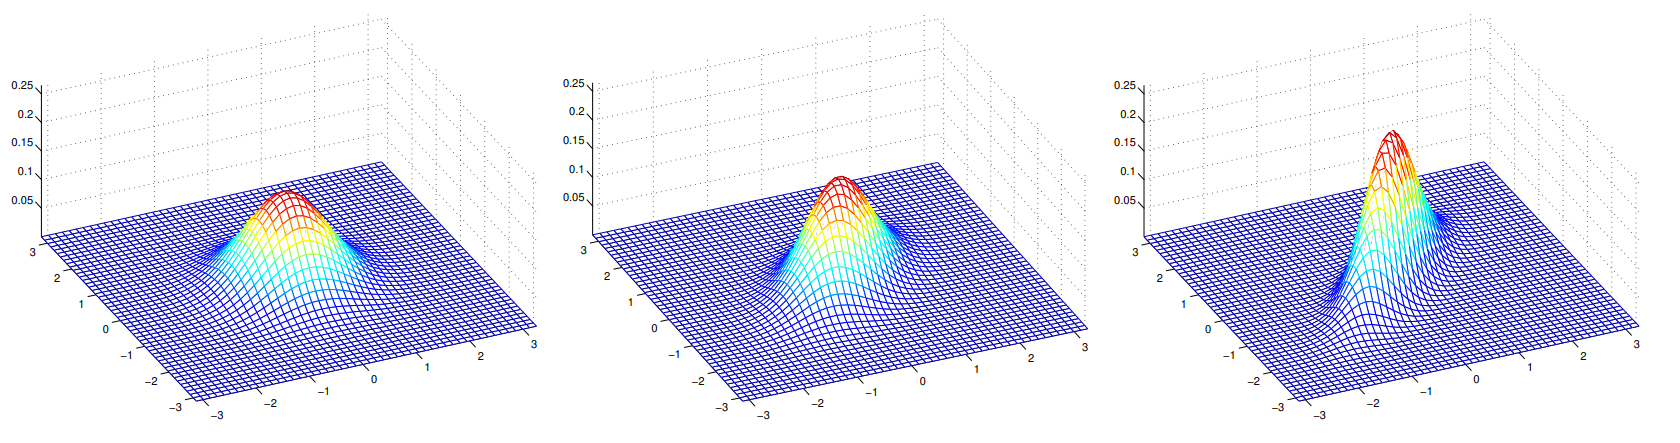
\includegraphics[width=1.0\linewidth]{figs/gaussian_density2.png}
\end{figure}

上面的图显示了均值为 0、协方差矩阵分别为
\[
    \Sigma = \begin{bmatrix} &1& &0& \\ &0& &1& \end{bmatrix}; \Sigma = \begin{bmatrix} &1& &0.5& \\ &0.5& &1& \end{bmatrix}; \Sigma = \begin{bmatrix} &1& &0.8& \\ &0.8& &1& \end{bmatrix}.
\]
最左边的图显示的是熟悉的标准正态分布,并且可以看到,随着 $\Sigma$ 中非对角线元素的增加,密度函数变得更加“压缩”到 $45^\circ$ 线(由 $x_1 = x_2$ 给出)。当观察这三个密度函数的等高线时,可以更清楚地看到这一点:

\begin{figure}[H]
    \centering
    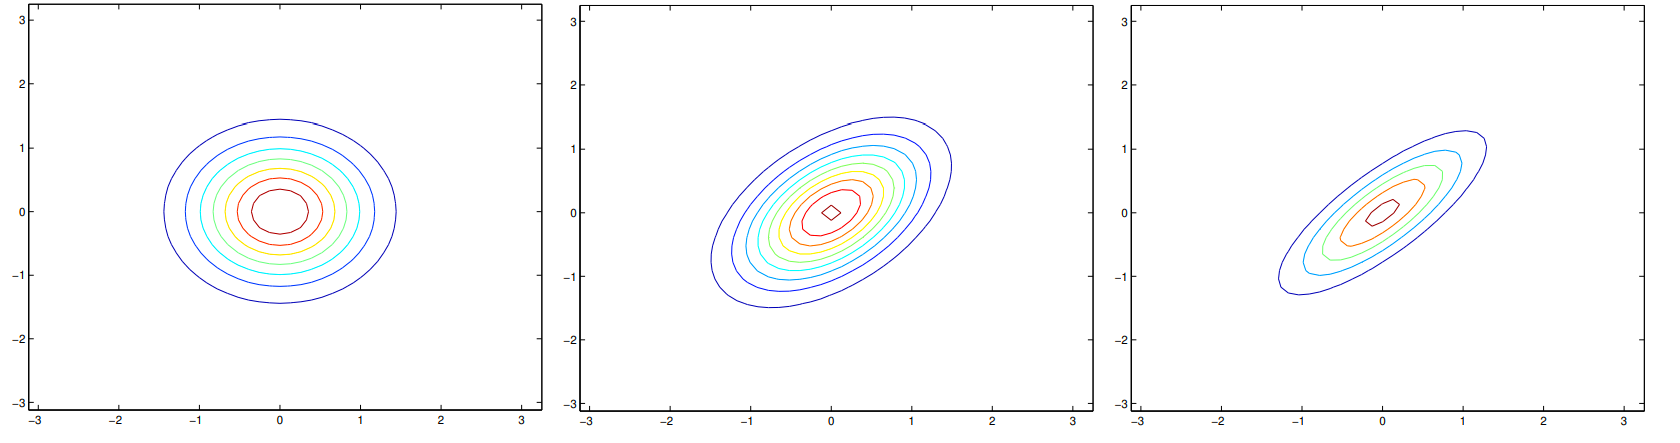
\includegraphics[width=1.0\linewidth]{figs/gaussian_contour1.png}
\end{figure}

下面是另外一组由不同的 $\Sigma$ 生成的例子:

\begin{figure}[H]
    \centering
    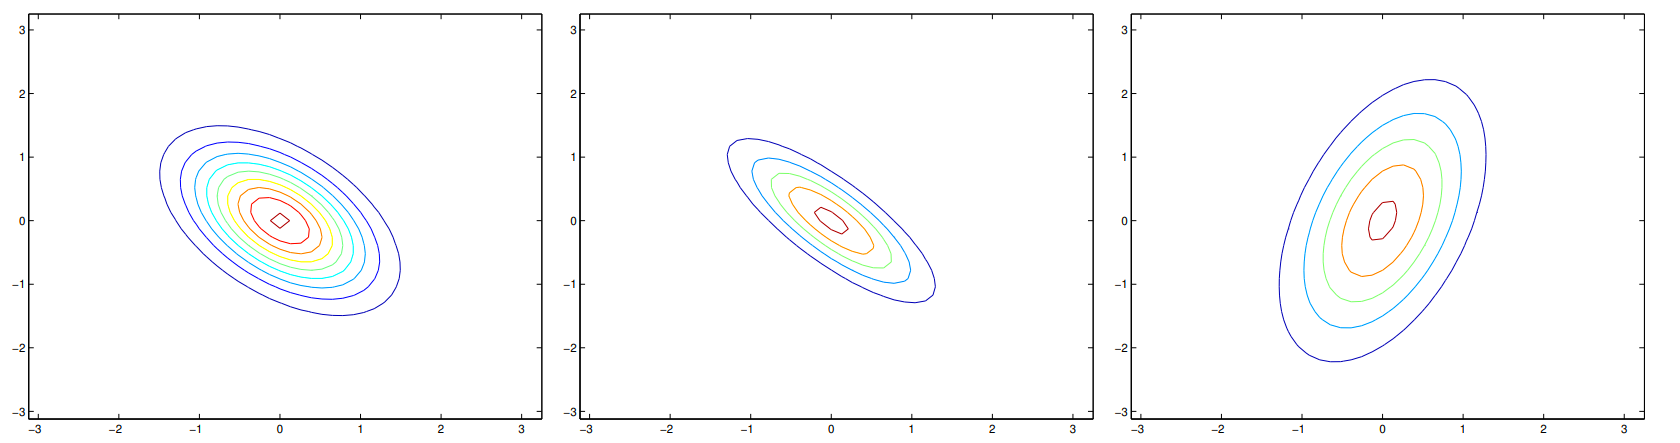
\includegraphics[width=1.0\linewidth]{figs/gaussian_contour2.png}
\end{figure}

上面的图分别使用了
\[
    \Sigma = \begin{bmatrix} &1& &-0.5& \\ &-0.5& &1& \end{bmatrix}; \Sigma = \begin{bmatrix} &1& &-0.8& \\ &-0.8& &1& \end{bmatrix}; \Sigma = \begin{bmatrix} &3& &0.8& \\ &0.8& &1& \end{bmatrix}.
\]
从最左边和中间的图可以看到,通过减小协方差矩阵的非对角线元素,密度函数再次变得“压缩”,但方向相反。最后值得一提的是,当改变参数时,等高线通常会形成椭圆(最右边的图显示了一个例子)。

作为最后一组例子,通过固定 $\Sigma = I$,并改变 $\mu$,也可以移动密度函数的均值。

\begin{figure}[H]
    \centering
    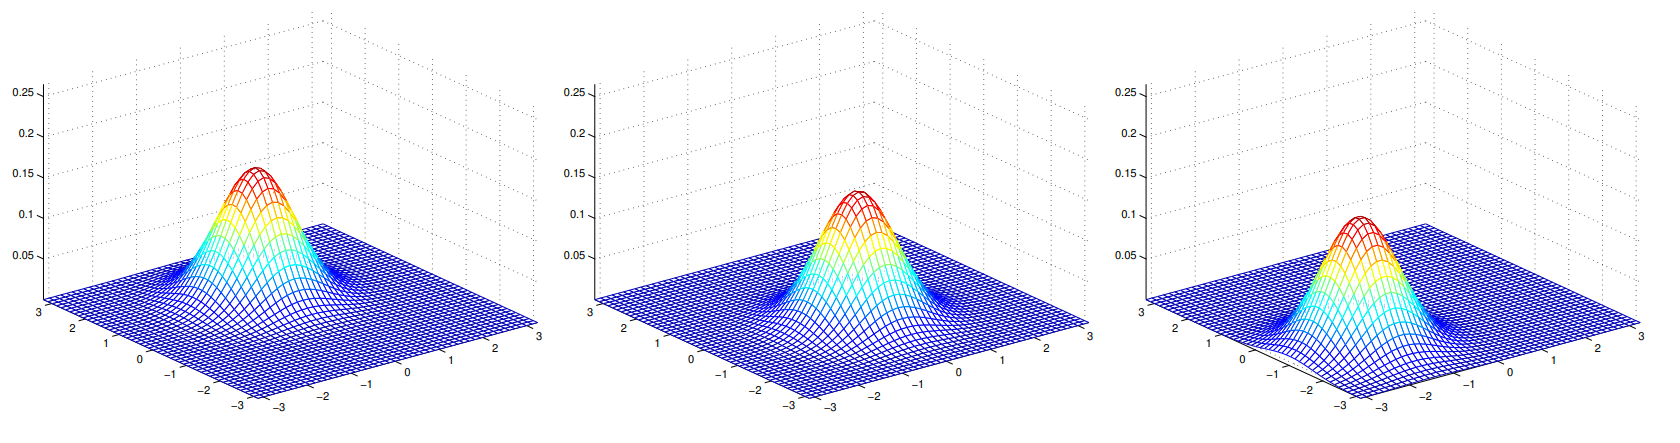
\includegraphics[width=1.0\linewidth]{figs/gaussian_density3.png}
\end{figure}

上面的图是使用 $\Sigma = I$ 生成的,并且 $\mu$ 分别为
\[
    \mu = \begin{bmatrix} &1& \\ &0& \end{bmatrix}; \mu = \begin{bmatrix} &-0.5& \\ &0& \end{bmatrix}; \mu = \begin{bmatrix} &-1& \\ &-1.5& \end{bmatrix}.
\]

\subsection{高斯判别分析模型}

当遇到输入特征 $x$ 是连续随机变量的分类问题时,可以使用高斯判别分析模型,该模型利用多元正态分布对 $p(x|y)$ 进行建模。模型如下:
\[
\begin{aligned}
    y &\sim \text{Bernoulli}(\phi) \\
    x|y=0 &\sim \mathcal{N}(\mu_0, \Sigma) \\
    x|y=1 &\sim \mathcal{N}(\mu_1, \Sigma)
\end{aligned}
\]
写出分布形式为:
\[
\begin{aligned}
    p(y) &= \phi^y (1-\phi)^{1-y} \\
    p(x|y=0) &= \frac{1}{(2\pi)^{d/2}|\Sigma|^{1/2}} \exp\left(-\frac{1}{2}(x-\mu_0)^T \Sigma^{-1} (x-\mu_0)\right) \\
    p(x|y=1) &= \frac{1}{(2\pi)^{d/2}|\Sigma|^{1/2}} \exp\left(-\frac{1}{2}(x-\mu_1)^T \Sigma^{-1} (x-\mu_1)\right)
\end{aligned}
\]
模型中的参数为 $\phi, \Sigma, \mu_0$ 和 $\mu_1$。(注意,尽管有两个不同的均值向量 $\mu_0$ 和 $\mu_1$,但该模型通常只使用一个协方差矩阵 $\Sigma$。) 数据的对数似然函数如下:
\[
\begin{aligned}
    \ell(\phi, \mu_0, \mu_1, \Sigma) &= \log \prod_{i=1}^n p(x^{(i)}, y^{(i)}; \phi, \mu_0, \mu_1, \Sigma) \\
    &= \log \prod_{i=1}^n p(x^{(i)}|y^{(i)}; \mu_0, \mu_1, \Sigma) p(y^{(i)}; \phi).
\end{aligned}
\]

通过最大化 $\ell$ 对参数进行估计,可以得到参数的最大似然估计(参见习题集 1):
\[
\begin{aligned}
    \phi &= \frac{1}{n} \sum_{i=1}^n 1\{y^{(i)} = 1\} \\
    \mu_0 &= \frac{\sum_{i=1}^n 1\{y^{(i)} = 0\}x^{(i)}}{\sum_{i=1}^n 1\{y^{(i)} = 0\}} \\
    \mu_1 &= \frac{\sum_{i=1}^n 1\{y^{(i)} = 1\}x^{(i)}}{\sum_{i=1}^n 1\{y^{(i)} = 1\}} \\
    \Sigma &= \frac{1}{n} \sum_{i=1}^n (x^{(i)} - \mu_{y^{(i)}})(x^{(i)} - \mu_{y^{(i)}})^T.
\end{aligned}
\]

从直观上看,算法的操作可以表示如下:

\begin{figure}[H]
    \centering
    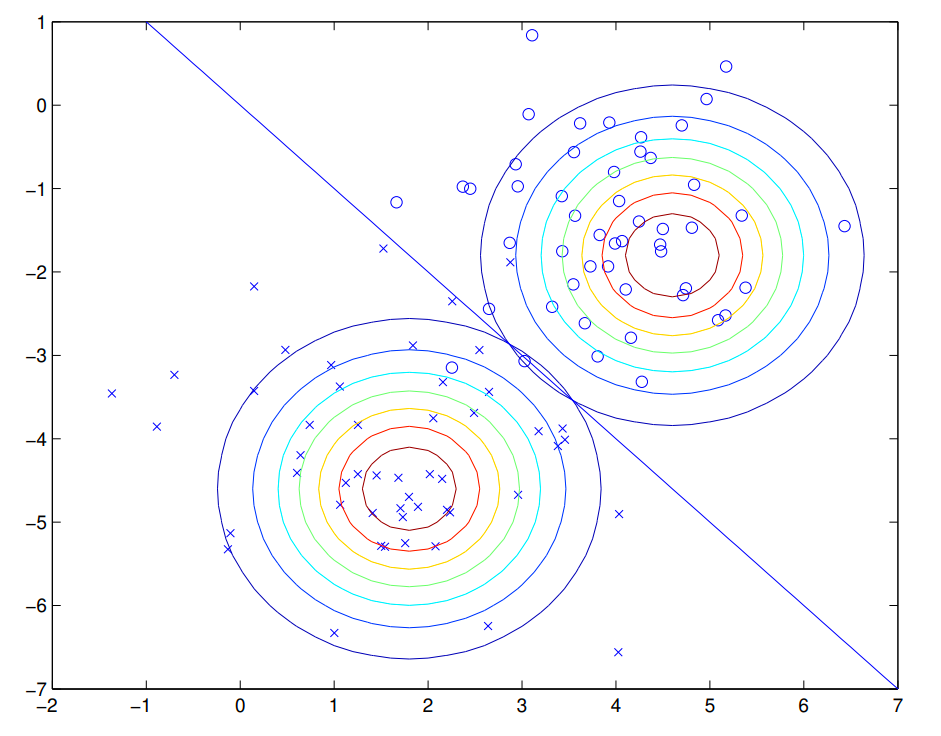
\includegraphics[width=0.5\linewidth]{figs/gda.png}
\end{figure}

图中展示了训练集以及拟合到两个类别数据的两个高斯分布的等高线。注意到由于共享协方差矩阵 $\Sigma$,这两个高斯分布的等高线形状和方向相同,但它们的均值 $\mu_0$ 和 $\mu_1$ 不同。图中还展示了 $p(y=1|x)=0.5$ 的决策边界直线。在边界的一侧,预测 $y=1$ 是最可能的结果,而在另一侧,则更多地预测 $y=0$。

\subsection{讨论:GDA 与逻辑回归}

GDA 模型与逻辑回归有着有趣的关系。如果将 $p(y=1|x; \phi, \mu_0, \mu_1, \Sigma)$ 视为 $x$ 的函数,会发现它可以表示为以下形式:
\[
    p(y=1|x; \phi, \mu_0, \mu_1, \Sigma) = \frac{1}{1+\exp(-\theta^T x)},
\]
其中 $\theta$ 是 $\phi, \mu_0, \mu_1, \Sigma$ 的适当函数。\footnote{这里采用了重新定义右侧 $x^{(i)}$ 为 $(d+1)$ 维向量的约定,即添加额外的坐标 $x_0^{(i)} = 1$;参见习题集 1。} 这正是逻辑回归(一种判别式算法)用来建模 $p(y=1|x)$ 的形式。

何时应该优先选择其中一个模型,何时又该选择另一个?GDA 和逻辑回归在同一数据集上训练时,通常会给出不同的决策边界,如何判断哪个会更好?

前文论述了,如果 $p(x|y)$ 是多元高斯分布(且共享 $\Sigma$),那么 $p(y|x)$ 必然是逻辑函数。反之则不成立,即 $p(y|x)$ 是逻辑函数并不意味着 $p(x|y)$ 是多元高斯分布。这表明 GDA 对数据做出了比逻辑回归更强的建模假设。事实证明,当这些建模假设正确时,GDA 会更好地拟合数据,并且是一个更好的模型。具体来说,当 $p(x|y)$ 确实是高斯分布(且共享 $\Sigma$)时,GDA 具有\textbf{渐近效率 (asymptotically efficient)}。非正式地讲,这意味着在训练集非常大($n$ 很大)的极限情况下,没有哪个算法能比 GDA 更好(例如,在估计 $p(y|x)$ 的准确性方面)。特别地,在这种情况下,可以证明 GDA 是比逻辑回归更好的算法;更一般地,即使训练集较小,通常也期望 GDA 表现更好。

相比之下,通过做出显著较弱的假设,逻辑回归也更\textit{鲁棒 (Robust)},对不正确的建模假设更不敏感。有许多不同的假设集合可以导致 $p(y|x)$ 呈现逻辑函数的形式。例如,如果 $x|y=0 \sim \text{Poisson}(\lambda_0)$ 且 $x|y=1 \sim \text{Poisson}(\lambda_1)$,那么 $p(y|x)$ 将是逻辑函数。逻辑回归在这种泊松分布数据上也能很好地工作。但是,如果对非高斯数据使用 GDA 并拟合高斯分布,那么结果将不太可预测,并且 GDA 可能表现不佳。

总结来说:GDA 做出了更强的建模假设,并且在建模假设正确或至少近似正确时,数据效率更高(即,需要较少的训练数据来“很好地”学习)。逻辑回归做出了较弱的假设,并且对建模假设的错误更鲁棒。具体来说,当数据确实是非高斯分布时,在大数据集的极限情况下,逻辑回归几乎总是比 GDA 表现更好。因此,在实践中,逻辑回归比 GDA 使用更频繁。(关于判别式模型与生成式模型的某些相关考虑也适用于接下来讨论的朴素贝叶斯算法,但朴素贝叶斯算法仍然被认为是一个非常好的,并且当然也是一个非常流行的分类算法。)

\section{朴素贝叶斯(选读)}

在 GDA 中,特征向量 $x$ 是连续的实值向量。接下来讨论一种不同的学习算法,其中 $x_j$ 是离散值。

以构建电子邮件垃圾邮件过滤器为例,考虑使用机器学习。希望根据消息是否为未经请求的商业(垃圾邮件)或非垃圾邮件来对其进行分类。学习完成后,可以使邮件阅读器自动过滤掉垃圾邮件,并将其放入单独的文件夹中。对电子邮件进行分类是更广泛的问题集合(称为\textbf{文本分类 (text classification)})的一个示例。

假设有一个训练集(一组标记为垃圾邮件或非垃圾邮件的电子邮件)。首先通过指定用于表示电子邮件的特征 $x_j$ 来构建垃圾邮件过滤器。

将通过一个特征向量来表示一封电子邮件,该向量的长度等于字典中的单词数量。具体来说,如果一封电子邮件包含字典中的第 $j$ 个单词,则设置 $x_j=1$;否则,设置 $x_j=0$。例如,以下向量:


\[
x = 
\begin{bmatrix}
    &1& \\
    &0& \\
    &0& \\
    &\vdots& \\
    &1& \\
    &\vdots& \\
    &0&
\end{bmatrix}
\quad % 或者 \qquad 调整间距
\begin{array}{l}
    \text{a} \\
    \text{aardvark} \\
    \text{aardwolf} \\
    \vdots \\
    \text{buy} \\
    \vdots \\
    \text{zygmurgy}
\end{array}
\]
表示一封包含单词“a”和“buy”但不包含“aardvark”、“aardwolf”或“zygmurgy”的电子邮件。\footnote{实际上,在实践中会查看训练集并仅将至少出现一次的单词编码到特征向量中,而不是查看所有英文单词的列表。除了减少建模的单词数量,从而降低计算和空间需求外,这还有一个优点,即允许对可能出现在电子邮件中(例如“cs229”)但在字典中找不到的许多单词进行建模/包含作为特征。有时(在作业中)还会排除非常高频的单词(例如“the”、“of”和“and”);这些高频的“无内容”词被称为\textbf{停用词 (stop words)},因为它们在许多文档中都会出现,并且很少能表明电子邮件是垃圾邮件还是非垃圾邮件。} 用于编码特征向量的单词集合称为\textbf{词汇表 (vocabulary)},因此 $x$ 的维度等于词汇表的大小。

在选择了特征向量之后,现在希望构建一个生成模型。因此,需要对 $p(x|y)$ 进行建模。但是,如果词汇表有 50000 个单词,那么 $x \in \{0, 1\}^{50000}$($x$ 是一个由 0 和 1 组成的 50000 维向量),如果对 $x$ 使用 2$^{50000}$ 种可能结果的多项分布进行显式建模,最终会得到一个 $(2^{50000}-1)$ 维参数向量。参数数量显然太多了。

因此,为了对 $p(x|y)$ 进行建模,将做出一个非常强的假设。假设给定 $y$ 时,$x_i$ 是条件独立的。这个假设称为\textbf{朴素贝叶斯假设 (Naive Bayes (NB) assumption)},由此产生的算法称为\textbf{朴素贝叶斯分类器 (Naive Bayes classifier)}。例如,如果 $y=1$ 表示垃圾邮件,“buy”是第 2087 个单词,“price”是第 39831 个单词;那么假设如果知道 $y=1$(这封特定的电子邮件是垃圾邮件),那么关于 $x_{2087}$ 的知识(消息中是否出现“buy”)对关于 $x_{39831}$ 的值(是否出现“price”)的信念没有影响。更正式地讲,这可以写成 $p(x_{2087}|y) = p(x_{2087}|y, x_{39831})$。(注意,这与 $x_{2087}$ 和 $x_{39831}$ 是独立的说法不同,独立的说法会写成 $p(x_{2087}) = p(x_{2087}|x_{39831})$;相反,这里只假设给定 $y$ 时,$x_{2087}$ 和 $x_{39831}$ 是条件独立的。)

现在有:
\[
    \begin{aligned}
        p(x_1, \dots, x_{50000}|y) &= p(x_1|y)p(x_2|y, x_1)p(x_3|y, x_1, x_2) \cdots p(x_{50000}|y, x_1, \dots, x_{49999}) \\ 
        &= p(x_1|y)p(x_2|y)p(x_3|y) \cdots p(x_{50000}|y) \\ 
        &= \prod_{j=1}^d p(x_j|y) 
    \end{aligned}
\]
第一个等号仅遵循概率的通常性质,第二个等号使用了朴素贝叶斯假设。注意,尽管朴素贝叶斯假设是一个非常强的假设,但由此产生的算法在许多问题上效果很好。

模型由 $\phi_{j|y=1} = p(x_j=1|y=1)$、$\phi_{j|y=0} = p(x_j=1|y=0)$ 和 $\phi_y = p(y=1)$ 参数化。像往常一样,给定训练集 $\{(x^{(i)}, y^{(i)}); i=1, \dots, n\}$,可以写出数据的联合似然:
\[
    \mathcal{L}(\phi_y, \phi_{j|y=0}, \phi_{j|y=1}) = \prod_{i=1}^n p(x^{(i)}, y^{(i)}).
\]
关于 $\phi_y$、$\phi_{j|y=0}$ 和 $\phi_{j|y=1}$ 最大化此式,得到最大似然估计:
\[
    \begin{aligned}
        \phi_{j|y=1} &= \frac{\sum_{i=1}^n {1}\{x_j^{(i)} = 1 \wedge y^{(i)} = 1\}}{\sum_{i=1}^n {1}\{y^{(i)} = 1\}} \\ 
        \phi_{j|y=0} &= \frac{\sum_{i=1}^n {1}\{x_j^{(i)} = 1 \wedge y^{(i)} = 0\}}{\sum_{i=1}^n {1}\{y^{(i)} = 0\}} \\ 
        \phi_y &= \frac{\sum_{i=1}^n {1}\{y^{(i)} = 1\}}{n} 
    \end{aligned}
\]
在上面的公式中,“$\wedge$”符号表示“逻辑且”。参数具有非常自然的解释。例如,$\phi_{j|y=1}$ 是单词 $j$ 出现在垃圾邮件 ($y=1$) 中的比例。

在拟合了所有这些参数之后,为了对具有特征 $x$ 的新示例进行预测,只需计算:
\[
\begin{aligned}
    p(y=1|x) &= \frac{p(x|y=1)p(y=1)}{p(x)} \\
    &= \frac{\left(\prod_{j=1}^d p(x_j|y=1)\right) p(y=1)}{\left(\prod_{j=1}^d p(x_j|y=1)\right) p(y=1) + \left(\prod_{j=1}^d p(x_j|y=0)\right) p(y=0)},
\end{aligned}
\]
并选择后验概率较高的类别。

最后,注意,虽然主要针对特征 $x_j$ 是二值的问题开发了朴素贝叶斯算法,但可以很直接地将其推广到 $x_j$ 可以取 $\{1, 2, \dots, k_j\}$ 中的值,只需将 $p(x_j|y)$ 建模为多项分布而不是伯努利分布。实际上,即使某些原始输入属性(例如,之前示例中的房屋居住面积)是连续值,通常也会将其\textbf{离散化 (discretize)}——即将其转换为一小组离散值,然后应用朴素贝叶斯。例如,如果使用某个特征 $x_j$ 来表示居住面积,可以将连续值离散化如下:

\begin{table}[H]
    \centering
    \begin{tabular}{c|c|c|c|c|c}
        居住面积 (平方英尺) & < 400 & 400-800 & 800-1200 & 1200-1600 & > 1600 \\
        \hline
        $x_i$ & 1 & 2 & 3 & 4 & 5 
    \end{tabular}
\end{table}

因此,对于居住面积为 890 平方英尺的房屋,可以将相应的特征 $x_j$ 的值设置为 3。然后可以应用朴素贝叶斯算法,并如前所述,使用多项分布对 $p(x_j|y)$ 进行建模。当原始的连续值属性无法通过多元正态分布很好地建模时,离散化特征并使用朴素贝叶斯(而不是 GDA)通常会产生更好的分类器。

\subsection{拉普拉斯平滑}

如前所述,朴素贝叶斯算法在许多问题上效果相当不错,但有一个简单的修改可以使其效果更好,尤其是在文本分类方面。简要讨论一下该算法当前形式存在的问题,然后讨论如何解决它。

考虑垃圾邮件/电子邮件分类,假设于 20xx 年,在您 CS229 结课并出色地完成了项目后,您决定在 20xx 年 5 月左右提交您的工作以在 NeurIPS 会议上发表。\footnote{NeurIPS 是顶级机器学习会议之一。提交论文的截止日期通常在五月至六月。} 因为会在电子邮件中讨论该会议,所以您也开始收到包含“neurips”一词的消息。但这是您的第一篇 NeurIPS 论文,在此之前,您从未见过包含“neurips”一词的电子邮件;特别是在垃圾邮件/非垃圾邮件训练集中,“neurips”从未出现过。假设“neurips”是字典中的第 35000 个单词,您的朴素贝叶斯垃圾邮件过滤器会选择其最大似然估计参数 $\phi_{35000|y}$ 为:

\begin{align*} 
\phi_{35000|y=1} &= \frac{\sum_{i=1}^n {1}\{x_{35000}^{(i)} = 1 \wedge y^{(i)} = 1\}}{\sum_{i=1}^n {1}\{y^{(i)} = 1\}} = 0 \\ \phi_{35000|y=0} &= \frac{\sum_{i=1}^n {1}\{x_{35000}^{(i)} = 1 \wedge y^{(i)} = 0\}}{\sum_{i=1}^n {1}\{y^{(i)} = 0\}} = 0 
\end{align*}
也就是说,由于它从未在垃圾邮件或非垃圾邮件训练示例中见过“neurips”,它认为在任何类型的电子邮件中看到它的概率为零。因此,当尝试判断这些包含“neurips”的消息是否是垃圾邮件时,它会计算类别后验概率,并得到
\[
    p(y=1|x) = \frac{\prod_{j=1}^d p(x_j|y=1) p(y=1)}{\prod_{j=1}^d p(x_j|y=1) p(y=1) + \prod_{j=1}^d p(x_j|y=0) p(y=0)} = \frac{0}{0}.
\]
这是因为 $\prod_{j=1}^d p(x_j|y)$ 的每一项都包含一个 $p(x_{35000}|y) = 0$ 的项,该项与乘积相乘。因此,算法得到 0/0,无法做出预测。

更广泛地说,仅仅因为在有限的训练集中没有看到某个事件,就将其概率估计为零,这在统计上是一个糟糕的主意。考虑估计一个多项随机变量 $z$ 取值为 $\{1, \dots, k\}$ 的问题。可以用 $\phi_j = p(z=j)$ 参数化多项分布。给定一组 $n$ 个独立观测值 $\{z^{(1)}, \dots, z^{(n)}\}$,最大似然估计由下式给出:
\[
    \phi_j = \frac{\sum_{i=1}^n {1}\{z^{(i)} = j\}}{n}.
\]
正如之前看到的,如果使用这些最大似然估计,那么一些 $\phi_j$ 可能会变为零,这是一个问题。为了避免这种情况,可以使用\textbf{拉普拉斯平滑 (Laplace smoothing)},它将上述估计替换为:
\[
    \phi_j = \frac{1 + \sum_{i=1}^n {1}\{z^{(i)} = j\}}{k + n}.
\]
在这里,在分子中加了 1,在分母中加了 $k$。注意,$\sum_{j=1}^k \phi_j = 1$ 仍然成立(自己验证一下!),这是一个理想的属性,因为 $\phi_j$ 是概率的估计,而概率之和必须为 1。此外,对于所有 $j$ 的值,$\phi_j \ne 0$,解决了概率估计为零的问题。在某些(可以说相当强的)条件下,可以证明拉普拉斯平滑实际上给出了 $\phi_j$ 的最优估计。

回到朴素贝叶斯分类器,使用拉普拉斯平滑,因此得到以下参数估计:
\begin{align*} \phi_{j|y=1} &= \frac{1 + \sum_{i=1}^n {1}\{x_j^{(i)} = 1 \wedge y^{(i)} = 1\}}{2 + \sum_{i=1}^n {1}\{y^{(i)} = 1\}} \\ \phi_{j|y=0} &= \frac{1 + \sum_{i=1}^n {1}\{x_j^{(i)} = 1 \wedge y^{(i)} = 0\}}{2 + \sum_{i=1}^n {1}\{y^{(i)} = 0\}} \end{align*}
(在实践中,是否对 $\phi_y$ 应用拉普拉斯平滑通常无关紧要,因为通常垃圾邮件和非垃圾邮件的比例都相当可观,所以 $\phi_y$ 将是 $p(y=1)$ 的合理估计,并且无论如何都会远离 0。)

\subsection{文本分类的事件模型}

为了结束关于生成学习算法的讨论,下面讨论一个专门用于文本分类的模型。虽然前面介绍的朴素贝叶斯在许多分类问题上效果很好,但对于文本分类,有一个相关的模型效果更好。

在文本分类的具体背景下,前面介绍的朴素贝叶斯使用了\textbf{伯努利事件模型 (Bernoulli event model)}(或有时称为\textbf{多元伯努利事件模型 (multi-variate Bernoulli event model)})。在该模型中,假设生成电子邮件的过程是:首先随机确定(根据类别先验 $p(y)$)发送者是垃圾邮件发送者还是非垃圾邮件发送者。然后,发送电子邮件的人遍历字典,独立地决定是否根据概率 $p(x_j=1|y) = \phi_{j|y}$ 在该电子邮件中包含每个单词 $j$。因此,消息的概率由 $p(y) \prod_{j=1}^d p(x_j|y)$ 给出。

这里有一个不同的模型,称为\textbf{多项事件模型 (Multinomial event model)}。为了描述该模型,将使用不同的表示法和特征集来表示电子邮件。令 $x_j$ 表示电子邮件中第 $j$ 个单词的标识。因此,$x_j$ 现在是一个整数,取值范围为 $\{1, \dots, |V|\}$,其中 $|V|$ 是词汇表(字典)的大小。包含 $d$ 个单词的电子邮件现在由一个长度为 $d$ 的向量 $(x_1, x_2, \dots, x_d)$ 表示;注意 $d$ 可以因不同的文档而异。例如,如果一封电子邮件以“A NeurIPS ...”开头,那么 $x_1=1$(“a”是字典中的第一个单词),$x_2=35000$(如果“neurips”是字典中的第 35000 个单词)。

在多项事件模型中,假设生成电子邮件的过程是一个随机过程,其中首先确定(根据 $p(y)$)是垃圾邮件还是非垃圾邮件,这与之前相同。然后,发送电子邮件的人通过首先从某个多项分布 $p(x_1|y)$ 生成 $x_1$ 来编写电子邮件。接下来,第二个单词 $x_2$ 独立于 $x_1$ 但来自相同的多项分布中选择,对于 $x_3, x_4$ 等也是如此,直到生成了电子邮件中的所有 $d$ 个单词。因此,消息的总概率由 $p(y) \prod_{j=1}^d p(x_j|y)$ 给出。注意,该公式看起来与之前在伯努利事件模型下消息概率的公式相同,但公式中的项现在表示完全不同的事物。特别是 $p(x_j|y)$ 现在是一个多项分布而非伯努利分布。

新模型的参数是 $\phi_y = p(y)$ 和 $\phi_{k|y=1} = p(x_j = k | y = 1)$(对于任何 $j$)以及 $\phi_{k|y=0} = p(x_j = k | y = 0)$。注意,假设 $p(x_j|y)$ 对于所有 $j$ 的值都是相同的(即,生成单词的分布不依赖于它在电子邮件中的位置 $j$)。

如果给定训练集 $\{(x^{(i)}, y^{(i)}); i=1, \dots, n\}$,其中 $x^{(i)} = (x_1^{(i)}, x_2^{(i)}, \dots, x_{d_i}^{(i)})$(此处,$d_i$ 是第 $i$ 个训练样本中的单词数),则数据的似然由下式给出:
\begin{align*}
    \mathcal{L}(\phi_y, \phi_{k|y=0}, \phi_{k|y=1}) &= \prod_{i=1}^n p(x^{(i)}, y^{(i)})\\
    &= \prod_{i=1}^n \left( \prod_{j=1}^{d_i} p(x_j^{(i)} | y^{(i)}; \phi_{k|y=0}, \phi_{k|y=1}) \right) p(y^{(i)}; \phi_y).
\end{align*}

最大化此似然得到参数的最大似然估计:
\begin{align*} 
    \phi_{k|y=1} &= \frac{\sum_{i=1}^n \sum_{j=1}^{d_i} {1}\{x_j^{(i)} = k \wedge y^{(i)} = 1\}}{\sum_{i=1}^n {1}\{y^{(i)} = 1\} d_i} \\ 
    \phi_{k|y=0} &= \frac{\sum_{i=1}^n \sum_{j=1}^{d_i} {1}\{x_j^{(i)} = k \wedge y^{(i)} = 0\}}{\sum_{i=1}^n {1}\{y^{(i)} = 0\} d_i} \\ 
    \phi_y &= \frac{\sum_{i=1}^n {1}\{y^{(i)} = 1\}}{n}. 
\end{align*}
如果对估计 $\phi_{k|y=0}$ 和 $\phi_{k|y=1}$ 应用拉普拉斯平滑(在实践中为了获得良好性能是必需的),在分子中加 1,在分母中加 $|V|$,得到:
\begin{align*} 
    \phi_{k|y=1} &= \frac{1 + \sum_{i=1}^n \sum_{j=1}^{d_i} {1}\{x_j^{(i)} = k \wedge y^{(i)} = 1\}}{|V| + \sum_{i=1}^n {1}\{y^{(i)} = 1\} d_i} \\ 
    \phi_{k|y=0} &= \frac{1 + \sum_{i=1}^n \sum_{j=1}^{d_i} {1}\{x_j^{(i)} = k \wedge y^{(i)} = 0\}}{|V| + \sum_{i=1}^n {1}\{y^{(i)} = 0\} d_i}. 
\end{align*}
虽然朴素贝叶斯分类器不一定是最好的分类算法,但它通常效果出奇地好。考虑到其简单性和易于实现性,它通常也是一个非常好的“第一步”尝试。

\chapter{核方法}

\section{特征映射}

回顾在线性回归的讨论中,考虑了根据房屋的居住面积(记为 $x$)预测房屋价格(记为 $y$)的问题,并将 $x$ 的线性函数拟合到训练数据。如果价格 $y$ 可以更准确地表示为 $x$ 的\textit{非线性 (non-linear)}函数呢?在这种情况下,需要一个比线性模型更具表现力的模型族。

首先考虑拟合三次函数 $y = \theta_3 x^3 + \theta_2 x^2 + \theta_1 x + \theta_0$。结果表明,可以将三次函数视为在不同特征变量集(定义如下)上的线性函数。具体来说,令函数 $\phi: \mathbb{R} \to \mathbb{R}^4$ 定义为
\begin{equation}
    \phi(x) = \begin{bmatrix} &1& \\ &x& \\ &x^2& \\ &x^3& \end{bmatrix} \in \mathbb{R}^4.
    \label{eq:kernel_phi}
\end{equation}

令 $\theta \in \mathbb{R}^4$ 是包含 $\theta_0, \theta_1, \theta_2, \theta_3$ 作为元素的向量。那么可以将三次函数写成 $x$ 的形式:
\[
    \theta_3 x^3 + \theta_2 x^2 + \theta_1 x + \theta_0 = \theta^T \phi(x).
\]
因此,变量 $x$ 的三次函数可以视为变量 $\phi(x)$ 上的线性函数。为了区分这两组变量,在核方法的背景下,将问题的“原始”输入值称为输入\textbf{属性 (attributes)}(在本例中为 $x$,即居住面积)。当原始输入被映射到一组新的量 $\phi(x)$ 时,将这些新的量称为\textbf{特征 (features)} 变量。(不幸的是,不同的作者在不同的语境下使用不同的术语来描述这两者。)将 $\phi$ 称为\textbf{特征映射 (feature map)},它将属性映射到特征。

\section{带特征的最小均方}

现在我们推导拟合模型 $\theta^T \phi(x)$ 的梯度下降算法。首先回顾一下,对于普通的最小二乘问题,拟合 $\theta^T x$ 的批量梯度下降更新(其推导参见讲义第一章)为:

\begin{align} 
    \theta &:= \theta + \alpha \sum_{i=1}^n (y^{(i)} - h_\theta(x^{(i)})) x^{(i)} \notag\\ 
    &:= \theta + \alpha \sum_{i=1}^n (y^{(i)} - \theta^T x^{(i)}) x^{(i)}.\label{eq:kernel_ols}
\end{align}

令 $\phi: \mathbb{R}^d \to \mathbb{R}^p$ 是一个将属性 $x$(在 $\mathbb{R}^d$ 中)映射到 $\mathbb{R}^p$ 中的特征 $\phi(x)$ 的特征映射。(在前面小节的示例中,$d=1$ 且 $p=4$。)现在目标是拟合函数 $\theta^T \phi(x)$,其中 $\theta$ 是 $\mathbb{R}^p$ 中的向量而不是 $\mathbb{R}^d$ 中的向量。可以将上面算法中 $x^{(i)}$ 的所有出现替换为 $\phi(x^{(i)})$,得到新的更新:
\begin{equation}
    \theta := \theta + \alpha \sum_{i=1}^n (y^{(i)} - \theta^T \phi(x^{(i)})) \phi(x^{(i)}).
    \label{eq:kernel_iterate}
\end{equation}
类似地,相应的随机梯度下降更新规则是
\begin{equation}
    \theta := \theta + \alpha (y^{(i)} - \theta^T \phi(x^{(i)})) \phi(x^{(i)}).
\end{equation}

\section{带核技巧的最小均方}

当特征 $\phi(x)$ 是高维时,上面的梯度下降或随机梯度下降更新在计算上变得昂贵。例如,考虑将方程 \eqref{eq:kernel_phi} 中的特征映射直接扩展到高维输入 $x$:假设 $x \in \mathbb{R}^d$,令 $\phi(x)$ 是包含所有 $x$ 的次数 $\le 3$ 的项的向量
\begin{equation}
    \phi(x) = \begin{bmatrix} &1& \\ &x_1& \\ &x_2& \\ &\vdots& \\ &x_1^2& \\ &x_1 x_2& \\ &x_1 x_3& \\ &\vdots& \\ &x_2 x_1& \\ &\vdots& \\ &x_1^3& \\ &x_1^2 x_2& \\ &\vdots& \\ &x_2 x_3 x_1& \\ &\vdots& \end{bmatrix}. \label{eq:5.5}
\end{equation}
特征 $\phi(x)$ 的维度大约是 $d^3$ 量级\footnote{此处,为简单起见,包含所有重复的单项式(因此,例如 $x_1 x_2 x_3$ 和 $x_2 x_3 x_1$ 都出现在 $\phi(x)$ 中)。因此,$\phi(x)$ 中共有 $1 + d + d^2 + d^3$ 个元素。}。对于计算来说,这是一个非常长的向量——当 $d = 1000$ 时,每次更新需要至少计算和存储一个 $1000^3 = 10^9$ 维向量,这比普通最小二乘更新规则 \eqref{eq:kernel_ols} 慢 $10^6$ 倍。

乍一看,每次更新 $d^3$ 的运行时长和内存使用似乎是不可避免的,因为向量 $\theta$ 本身的维度是 $p \approx d^3$,并且可能需要更新和存储 $\theta$ 的每一个元素。然而,将引入核技巧,通过它不需要显式存储 $\theta$,并且运行时长可以显著改善。

为简单起见,假设初始值 $\theta = 0$,并且关注迭代更新 \eqref{eq:kernel_iterate}。主要观察是,在任何时候,$\theta$ 都可以表示为向量 $\phi(x^{(1)}), \dots, \phi(x^{(n)})$ 的线性组合。实际上,可以通过归纳法证明如下。在初始化时,$\theta = 0 = \sum_{i=1}^n 0 \cdot \phi(x^{(i)})$。假设在某个时刻,$\theta$ 可以表示为
\begin{equation}
    \theta = \sum_{i=1}^n \beta_i \phi(x^{(i)}).
\end{equation}
其中 $\beta_1, \dots, \beta_n \in \mathbb{R}$。然后,断言在下一轮中,$\theta$ 仍然是 $\phi(x^{(1)}), \dots, \phi(x^{(n)})$ 的线性组合,因为
\begin{align} 
    \theta &:= \theta + \alpha \sum_{i=1}^n (y^{(i)} - \theta^T \phi(x^{(i)})) \phi(x^{(i)}) \notag\\ 
    &= \sum_{i=1}^n \beta_i \phi(x^{(i)}) + \alpha \sum_{i=1}^n (y^{(i)} - \theta^T \phi(x^{(i)})) \phi(x^{(i)}) \notag\\ 
    &= \sum_{i=1}^n \underbrace{(\beta_i + \alpha (y^{(i)} - \theta^T \phi(x^{(i)})))}_{\text{新的 } \beta_i} \phi(x^{(i)}). 
\end{align}
可以意识到,一般策略是通过一组系数 $\beta_1, \dots, \beta_n$ 隐式表示 $p$ 维向量 $\theta$。为了做到这一点,推导系数 $\beta_i$ 的更新规则。使用上面的方程,可以看到新的 $\beta_i$ 依赖于旧的 $\beta_i$
\begin{equation}
    \beta_i := \beta_i + \alpha (y^{(i)} - \theta^T \phi(x^{(i)})).
\end{equation}
这里,方程的右侧仍然有旧的 $\theta$。将 $\theta$ 替换为 $\theta = \sum_{j=1}^n \beta_j \phi(x^{(j)})$ 得到
\[
    \forall i \in \{1, \dots, n\}, \beta_i := \beta_i + \alpha \left( y^{(i)} - \sum_{j=1}^n \beta_j \phi(x^{(j)})^T \phi(x^{(i)}) \right).
\]
通常将 $\phi(x^{(j)})^T \phi(x^{(i)})$ 重写为 $\langle \phi(x^{(j)}), \phi(x^{(i)}) \rangle$ 以强调它是两个特征向量的内积。通过将 $\beta_i$ 视为 $\theta$ 的新表示,已经成功地将批梯度下降算法转化为一个迭代更新 $\beta$ 值的新算法。它可能看起来在每次迭代时,仍然需要计算所有 $i, j$ 对的 $\langle \phi(x^{(j)}), \phi(x^{(i)}) \rangle$ 的值,其中每个计算可能需要大约 $O(p)$ 的操作。然而,有两个重要的特性可以解决这个问题:
\begin{enumerate}
    \item 在循环开始之前,可以预先计算所有 $i, j$ 对的成对内积 $\langle \phi(x^{(j)}), \phi(x^{(i)}) \rangle$。
    \item 对于定义在 \eqref{eq:5.5} 中的特征映射 $\phi$(或许多其他有趣的特征映射),计算 $\langle \phi(x^{(j)}), \phi(x^{(i)}) \rangle$ 可以是高效的并且不必需显式计算 $\phi(x^{(i)})$。这是因为:
    \begin{align} 
        \langle \phi(x), \phi(z) \rangle &= 1 + \sum_{i=1}^d x_i z_i + \sum_{i,j \in \{1, \dots, d\}} x_i x_j z_i z_j + \sum_{i,j,k \in \{1, \dots, d\}} x_i x_j x_k z_i z_j z_k \notag\\ 
        &= 1 + \sum_{i=1}^d x_i z_i + \left( \sum_{i=1}^d x_i z_i \right)^2 + \left( \sum_{i=1}^d x_i z_i \right)^3 \notag\\ 
        &= 1 + \langle x, z \rangle + \langle x, z \rangle^2 + \langle x, z \rangle^3 \label{eq:5.9}
    \end{align}
    因此,要计算 $\langle \phi(x), \phi(z) \rangle$,可以首先用 $O(d)$ 的时间计算 $\langle x, z \rangle$,然后进行一些常数次操作来计算 $1 + \langle x, z \rangle + \langle x, z \rangle^2 + \langle x, z \rangle^3$。
\end{enumerate}

正如将看到的,特征 $\phi(x), \phi(z)$ 之间的内积在这里至关重要。将与特征映射 $\phi$ 对应的\textbf{核 (Kernel)}定义为一个 $\mathcal{X} \times \mathcal{X} \to \mathbb{R}$ 的函数,满足\footnote{回想一下, $\mathcal{X}$ 是输入 $x$ 的取值空间。在当前示例中,$\mathcal{X} = \mathbb{R}^d$。}:
\begin{equation}
    K(x, z) \triangleq \langle \phi(x), \phi(z) \rangle
\end{equation}

最终算法总结如下:

\noindent\hrulefill
\begin{enumerate}
    \item 使用方程 \eqref{eq:5.9} 计算所有 $i, j \in \{1, \dots, n\}$ 的值 $K(x^{(i)}, x^{(j)}) \triangleq \langle \phi(x^{(i)}), \phi(x^{(j)}) \rangle$。设置 $\beta := 0$。
    \item \textbf{循环}:
    \begin{equation}
        \forall i \in \{1, \dots, n\}, \beta_i := \beta_i + \alpha \left( y^{(i)} - \sum_{j=1}^n \beta_j K(x^{(i)}, x^{(j)}) \right).
        \label{eq:kernel_algo}
    \end{equation}
    或者用向量表示法,令 $K$ 是一个 $n \times n$ 矩阵,其中 $K_{ij} = K(x^{(i)}, x^{(j)})$,有
    \[
        \beta := \beta + \alpha (\vec{y} - K \beta)
    \]
\end{enumerate}
\hrulefill

通过上面的算法,可以在每次更新时以 $O(n)$ 的时间高效地更新向量 $\theta$ 的表示 $\beta$。最后,需要证明表示 $\beta$ 的知识足以计算预测 $\theta^T \phi(x)$。实际上,有
\begin{equation}
    \theta^T \phi(x) = \sum_{i=1}^n \beta_i \phi(x^{(i)})^T \phi(x) = \sum_{i=1}^n \beta_i K(x^{(i)}, x).
    \label{eq:kernel_essence}
\end{equation}
可以意识到,本质上所有需要知道的关于特征映射 $\phi(\cdot)$ 的信息都封装在相应的核函数 $K(\cdot, \cdot)$ 中。将在下一节中对此进行详细阐述。

\section{核的性质}

在上一小节中,从一个显式定义的特征映射 $\phi$ 开始,它导出了核函数 $K(x, z) \triangleq \langle \phi(x), \phi(z) \rangle$。然后,看到核函数是如此本质,只要核函数被定义,整个训练算法就可以完全用核方法的语言编写,而无需引用特征映射 $\phi$,因此对于测试示例 $x$ 的预测(方程 \eqref{eq:kernel_essence})也是如此。

因此,可以尝试定义其他核函数 $K(\cdot, \cdot)$ 并运行算法 \eqref{eq:kernel_algo}。请注意,算法 \eqref{eq:kernel_algo} 不需要显式访问特征映射 $\phi$,因此只需要确保特征映射 $\phi$ 的存在,但不一定需要能够显式写下 $\phi$。

哪些类型的函数 $K(\cdot, \cdot)$ 可以对应于某个特征映射 $\phi$? 换句话说,如果存在某个特征映射 $\phi$ 使得对于所有 $x, z$ 都有 $K(x, z) = \phi(x)^T \phi(z)$,能否判断出来?

如果可以通过给出有效核函数的精确表征来回答这个问题,那么就可以完全改变选择核函数 $K$ 的接口,而不是选择特征映射 $\phi$ 的接口。具体来说,可以选取一个函数 $K$,验证它满足该表征(从而存在一个与 $K$ 对应的特征映射 $\phi$),然后就可以运行更新规则 \eqref{eq:kernel_algo}。这里的好处是,不需要能够计算或解析地写下 $\phi$,只需要知道它的存在性。在本小节的末尾,在通过几个具体的核示例之后,将回答这个问题。

假设 $x, z \in \mathbb{R}^d$,首先考虑函数 $K(\cdot, \cdot)$ 定义为:
\[
    K(x, z) = (x^T z)^2.
\]
也可以将其写为
\begin{align} 
    K(x, z) &= \left( \sum_{i=1}^d x_i z_i \right) \left( \sum_{j=1}^d x_j z_j \right) \\ &= \sum_{i=1}^d \sum_{j=1}^d x_i x_j z_i z_j \\ &= \sum_{i,j=1}^d (x_i x_j)(z_i z_j) 
\end{align}
因此,可以看到 $K(x, z) = \langle \phi(x), \phi(z) \rangle$ 是与特征映射 $\phi$ 对应的核函数(这里以 $d=3$ 的情况为例)由下式给出
\[
    \phi(x) = \begin{bmatrix}
        &x_1 x_1& \\
        &x_1 x_2& \\
        &x_1 x_3& \\
        &x_2 x_1& \\
        &x_2 x_2& \\
        &x_2 x_3& \\
        &x_3 x_1& \\
        &x_3 x_2& \\
        &x_3 x_3&
    \end{bmatrix}.
\]
请回想一下核的计算效率,注意,虽然计算高维的 $\phi(x)$ 需要 $O(d^2)$ 的时间,但找到 $K(x, z)$ 只需 $O(d)$ 的时间——与输入属性的维度呈线性关系。

对于另一个相关的例子,也考虑由下式定义的 $K(\cdot, \cdot)$:
\[
    K(x, z) = (x^T z + c)^2
\]
\[
    = \sum_{i,j=1}^d (x_i x_j)(z_i z_j) + \sum_{i=1}^d (\sqrt{2c} x_i)(\sqrt{2c} z_i) + c^2.
\]
(请自行验证)这个函数 $K$ 是一个核函数,它对应到特征映射(再次以 $d=3$ 为例)
\[
    \phi(x) = \begin{bmatrix}
        &x_1 x_1& \\
        &x_1 x_2& \\
        &x_1 x_3& \\
        &x_2 x_1& \\
        &x_2 x_2& \\
        &x_2 x_3& \\
        &x_3 x_1& \\
        &x_3 x_2& \\
        &x_3 x_3& \\
        &\sqrt{2c} x_1& \\
        &\sqrt{2c} x_2& \\
        &\sqrt{2c} x_3& \\
        &c&
    \end{bmatrix},
\]
其中参数 $c$ 控制 $x_i$(一阶)项和 $x_i x_j$(二阶)项之间的相对权重。

更广泛地说,核 $K(x, z) = (x^T z + c)^k$ 对应于一个特征空间,包含所有次数不超过 $k$ 的一元多项式 $x_{i_1} x_{i_2} \dots x_{i_k}$。然而尽管在这个 $O(d^k)$ 维的高维空间中工作,计算 $K(x, z)$ 仍然只需要 $O(d)$ 的时间,因此即使在如此高维的特征空间中,也永远不需要显式表示出特征向量。

\subsection*{核作为相似性度量}

现在,讨论一下核的另一种视角。直观地(尽管这种直觉有一些问题,但先忽略),如果 $\phi(x)$ 和 $\phi(z)$ 彼此接近,那么可以期望 $K(x, z) = \phi(x)^T \phi(z)$ 很大。反过来,如果 $\phi(x)$ 和 $\phi(z)$ 相距很远——例如,几乎相互正交——那么 $K(x, z) = \phi(x)^T \phi(z)$ 将很小。因此,可以将 $K(x, z)$ 看作是 $\phi(x)$ 和 $\phi(z)$ 之间相似性的一种度量,或者说是 $x$ 和 $z$ 之间相似性的一种度量。

有了这种直觉,假设对于正在研究的某个学习问题,想出了一个函数 $K(x, z)$,认为它可能是衡量 $x$ 和 $z$ 相似性的合理度量。例如,可能选择了
\[
    K(x, z) = \exp \left( -\frac{\|x - z\|^2}{2\sigma^2} \right).
\]
这是衡量 $x$ 和 $z$ 相似性的合理度量,当 $x$ 和 $z$ 接近时接近 1,当 $x$ 和 $z$ 相距很远时接近 0。是否存在一个特征映射 $\phi$ 使得上面定义的核 $K$ 满足 $K(x, z) = \phi(x)^T \phi(z)$? 在这个特殊的例子中,答案是肯定的。这个核被称为\textbf{高斯核 (Gaussian kernel)},并且对应于一个无限维的特征映射 $\phi$。下面,我们将精确地描述一个函数 $K$ 需要满足哪些性质才能成为一个有效的核函数,即对应于某个特征映射 $\phi$。

\subsection*{有效核的必要条件}

现在假设 $K$ 确实是一个有效的核,对应于某个特征映射 $\phi$,首先看看它满足哪些性质。考虑一个包含 $n$ 个点(不一定是训练集)的有限集合 $\{x^{(1)}, \dots, x^{(n)}\}$,并定义一个 $n \times n$ 的方阵 $K$,其 $(i, j)$ 项由 $K_{ij} = K(x^{(i)}, x^{(j)})$ 给出。这个矩阵称为\textbf{核矩阵 (kernel matrix)}。请注意,我们为了方便使用了 $K$ 来表示核函数 $K(x, z)$ 和核矩阵 $K$,因为它们之间有明显的密切关系。

现在,如果 $K$ 是一个有效的核,那么 $K_{ij} = K(x^{(i)}, x^{(j)}) = \phi(x^{(i)})^T \phi(x^{(j)}) = \phi(x^{(j)})^T \phi(x^{(i)}) = K(x^{(j)}, x^{(i)}) = K_{ji}$,因此 $K$ 必须是对称的。此外,令 $\phi_k(x)$ 表示向量 $\phi(x)$ 的第 $k$ 个坐标,对于任意向量 $z$,有
\begin{align*} 
    z^T K z &= \sum_i \sum_j z_i K_{ij} z_j \\ 
    &= \sum_i \sum_j z_i \phi(x^{(i)})^T \phi(x^{(j)}) z_j \\ 
    &= \sum_i \sum_j z_i \left( \sum_k \phi_k(x^{(i)}) \phi_k(x^{(j)}) \right) z_j \\ 
    &= \sum_k \sum_i \sum_j z_i \phi_k(x^{(i)}) \phi_k(x^{(j)}) z_j \\ 
    &= \sum_k \left( \sum_i z_i \phi_k(x^{(i)}) \right) \left( \sum_j z_j \phi_k(x^{(j)}) \right) \\ 
    &= \sum_k \left( \sum_i z_i \phi_k(x^{(i)}) \right)^2 \\ 
    &\ge 0. 
\end{align*}
倒数第二步利用了 $\sum_{i,j} a_i a_j = (\sum_i a_i)^2$,其中 $a_i = z_i \phi_k(x^{(i)})$。由于 $z$ 是任意的,这表明 $K$ 是半正定的 ($K \ge 0$)。

因此,证明出,如果 $K$ 是一个有效的核(即,它对应于某个特征映射 $\phi$),那么相应的核矩阵 $K \in \mathbb{R}^{n \times n}$ 是对称半正定的。

\subsection*{有效核的充分条件}

更一般地,上面的条件不仅是必要的,而且也是 $K$ 成为有效核(也称为 Mercer 核)的充分条件。以下结果归功于 Mercer\footnote{许多文献以涉及 $L^2$ 函数的稍微更复杂的形式给出 Mercer 定理,但当输入属性取值为 $\mathbb{R}^d$ 时,这里给出的版本是等价的。}。

\noindent\textbf{定理(Mercer):} 设 $K: \mathbb{R}^d \times \mathbb{R}^d \mapsto \mathbb{R}$ 已知。则 $K$ 是一个有效核的充要条件是,对于任意有限集合 $\{x^{(1)}, \dots, x^{(n)}\}$ ($n < \infty$),相应的核矩阵是对称半正定的。

给定一个函数 $K$,除了尝试找到一个与之对应的特征映射 $\phi$ 之外,这个定理因此提供了另一种测试它是否是有效核的方法。在问题集 2 中也将有机会进一步探索这些想法。

课上还简要讨论了几个其他核的例子。例如,考虑手写数字识别问题,给定一个手写数字(0-9)的图像(16x16 像素),需要确定它是哪个数字。使用简单的多项式核 $K(x, z) = (x^T z)^k$ 或高斯核,SVM 能够在此问题上获得非常好的性能。这尤其令人惊讶,因为输入属性 $x$ 仅仅是图像像素值的 256 维向量,系统没有关于视觉的先验知识,甚至没有关于哪些像素相邻的知识。在课堂上简要讨论的另一个例子是,如果试图对字符串进行分类(例如,$x$ 是由氨基酸串成的蛋白质),那么构建一个合理、“小”的特征集对于大多数学习算法来说似乎很困难,特别是如果不同的字符串长度不同。然而,考虑让 $\phi(x)$ 是一个特征向量,它计算 $x$ 中每个长度为 $k$ 的子字符串的出现次数。如果考虑英文字母组成的字符串,那么有 $26^k$ 个这样的字符串。因此,$\phi(x)$ 是一个 $26^k$ 维向量;即使对于中等大小的 $k$,这可能也太大了,无法有效处理(例如,$26^4 \approx 460000$)。但是,使用(类似动态规划的)字符串匹配算法,可以有效地计算 $K(x, z) = \phi(x)^T \phi(z)$,这样就可以在这个 $26^k$ 维特征空间中隐式地工作,而无需显式计算特征向量。



\subsection*{核方法的应用}

已经看到了核方法在线性回归中的应用。在下一部分,将介绍支持向量机,核方法可以直接应用于其中。这里不再赘述。实际上,核方法的思想比线性回归和 SVM 具有更广泛的适用性。具体来说,如果有一个学习算法,可以完全用输入属性向量之间的内积 $\langle x, z \rangle$ 来表达,那么通过将其替换为核 $K(x, z)$(其中 $K$ 是一个核),就可以“神奇地”让算法在对应于 $K$ 的高维特征空间中高效工作。例如,这个核技巧可以应用于感知机,推导出核感知机算法。本课程后面将看到的许多算法也将适用于这种方法,这种方法被称为“核技巧”。

\chapter{支持向量机}

本章将介绍支持向量机(SVM)学习算法。SVM 是最好的(许多人甚至认为是最好的)“开箱即用”的监督学习算法之一。为了讲述 SVM 的故事,首先需要讨论间隔 (margin) 以及用大间隔分隔数据的思想。接下来,将讨论最优间隔分类器,这将引出对拉格朗日对偶性的讨论。还将看到核,它允许在非常高维(例如无限维)特征空间中高效地应用 SVM,最后会以 SMO 算法作为结束,该算法提供了 SVM 的高效实现。

\section{间隔:直觉}

我们将从讨论间隔开始讲述 SVM 的故事。本节将给出关于间隔以及预测的“置信度”的直觉;这些思想将在第 \ref{sec:6.3} 节中正式化。

考虑逻辑回归,其中概率 $p(y=1|x; \theta)$ 由 $h_\theta(x) = g(\theta^T x)$ 建模。当且仅当 $h_\theta(x) \ge 0.5$ 时,或者等价地,当且仅当 $\theta^T x \ge 0$ 时,预测输入 $x$ 的标签为“1”。考虑一个正训练样本 ($y=1$)。$\theta^T x$ 越大,$h_\theta(x) = p(y=1|x; \theta)$ 也越大,因此预测标签为 1 的“置信度”也越高。因此,可以非正式地认为,如果 $\theta^T x \gg 0$,则预测非常确信标签为 1。类似地,如果 $\theta^T x \ll 0$,则认为逻辑回归非常确信预测标签为 0。给定一个训练集,再次非正式地看来,如果能找到 $\theta$ 使得当 $y^{(i)}=1$ 时 $\theta^T x^{(i)} \gg 0$,并且当 $y^{(i)}=0$ 时 $\theta^T x^{(i)} \ll 0$,这将反映出一个非常确信(且正确)的分类集,其适用于所有训练样本。这似乎是一个很好的目标,很快将使用函数间隔的概念来形式化这个想法。

为了获得另一种直觉,考虑下面的图,其中 x 表示正训练样本,o 表示负训练样本,还显示了决策边界(这是由方程 $\theta^T x = 0$ 给出的直线,也称为\textbf{分隔超平面 (separating hyperplane)}),并且还标记了三个点 A、B 和 C。

\begin{figure}[H]
    \centering
    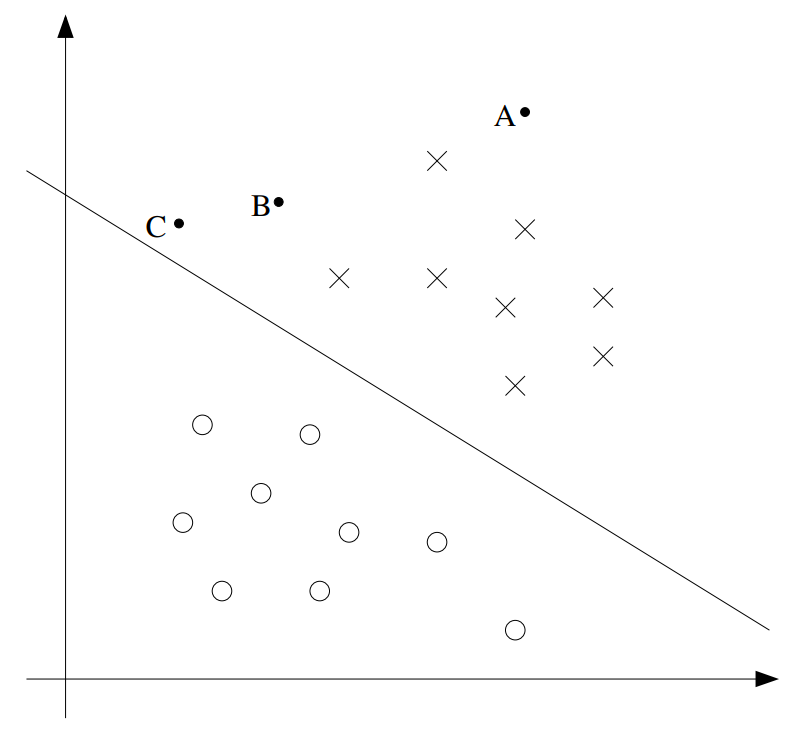
\includegraphics[width=0.5\linewidth]{figs/svm_hyperplane.png}
\end{figure}

注意到点 A 离决策边界非常远。如果要求预测 A 点的 $y$ 值,似乎应该非常确信那里 $y=1$。相反,点 C 离决策边界非常近,尽管它在决策边界预测 $y=1$ 的一侧,但决策边界的微小变化似乎很容易导致预测结果为 $y=0$。因此,在 A 点的预测比在 C 点更确信。点 B 介于这两种情况之间,更广泛地说,可以看出,如果一个点离分隔超平面很远,那么预测可能会更确信。同样,非正式地认为,如果给定一个训练集,能够找到一个决策边界,使得在训练样本上做出所有正确且确信(即远离决策边界)的预测,那将是很好的。稍后将使用几何间隔的概念来形式化这个想法。

\section{符号 (选读)}

为了更容易讨论 SVM,首先需要引入一种新的符号来讨论分类。将考虑一个二元分类问题的线性分类器,其标签为 $y$,特征为 $x$。从现在开始,使用 $y \in \{-1, 1\}$(而不是 $\{0, 1\}$)来表示类别标签。此外,不再使用向量 $\theta$ 来参数化线性分类器,而是使用参数 $w, b$,并将分类器写为
\[
    h_{w,b}(x) = g(w^T x + b).
\]
这里,$g(z) = 1$ 如果 $z \ge 0$,否则 $g(z) = -1$。这种“$w, b$”符号允许将截距项 $b$ 与其他参数分开处理(还放弃了之前让 $x_0 = 1$ 成为输入特征向量中的额外坐标的约定)。因此,$b$ 扮演着之前 $\theta_0$ 的角色,而 $w$ 扮演着 $[\theta_1 \dots \theta_d]^T$ 的角色。

还注意到,根据上面 $g$ 的定义,分类器将直接预测 1 或 -1(参见感知器算法),而无需先经过估计 $p(y=1)$ 的中间步骤(这是逻辑回归所做的)。

\section{函数间隔与几何间隔 (选读)}\label{sec:6.3}

现在将函数间隔和几何间隔的概念形式化。给定一个训练样本 $(x^{(i)}, y^{(i)})$,定义 $(w,b)$ 相对于训练样本的\textbf{函数间隔 (functional margin)}为
\[
    \hat{\gamma}^{(i)} = y^{(i)}(w^T x^{(i)} + b).
\]
注意,如果 $y^{(i)} = 1$,那么为了使函数间隔大(即,预测是确信且正确的),需要 $w^T x^{(i)} + b$ 是一个大的正数。相反,如果 $y^{(i)} = -1$,那么为了使函数间隔大,需要 $w^T x^{(i)} + b$ 是一个大的负数。此外,如果 $y^{(i)}(w^T x^{(i)} + b) > 0$,那么对这个样本的预测是正确的。(自己验证一下。)因此,大的函数间隔表示确信且正确的预测。

对于上面给出的 $g$ 选择的线性分类器(取值在 $\{-1, 1\}$ 中),然而函数间隔有一个性质使得它不是一个非常好的置信度度量。考虑 $g$ 的选择,注意到如果将 $w$ 替换为 $2w$,将 $b$ 替换为 $2b$,那么由于 $g(w^T x + b) = g(2w^T x + 2b)$,这根本不会改变 $h_{w,b}(x)$。也就是说,$g$,以及因此 $h_{w,b}(x)$,仅取决于 $w^T x + b$ 的符号,而不是大小。然而,将 $(w,b)$ 替换为 $(2w, 2b)$ 也会导致函数间隔乘以 2。因此,似乎通过利用缩放 $w$ 和 $b$ 的自由度,可以在不改变任何有意义的东西的情况下使函数间隔任意大。直观地说,因此施加某种归一化条件(例如 $||w||_2 = 1$)可能是有意义的;也就是说,可以将 $(w,b)$ 替换为 $(w/||w||_2, b/||w||_2)$,并改为考虑 $(w/||w||_2, b/||w||_2)$ 的函数间隔。稍后将回到这一点。

给定一个训练集 $S = \{(x^{(i)}, y^{(i)}); i = 1, \dots, n\}$,还定义 $(w,b)$ 相对于 $S$ 的函数间隔为各个训练样本的函数间隔中的最小值。用 $\hat{\gamma}$ 表示,因此可以写为:
\[
    \hat{\gamma} = \min_{i=1,\dots,n} \hat{\gamma}^{(i)}.
\]

接下来,讨论\textbf{几何间隔 (geometric margins)}。考虑下面的图:

\begin{figure}[H]
    \centering
    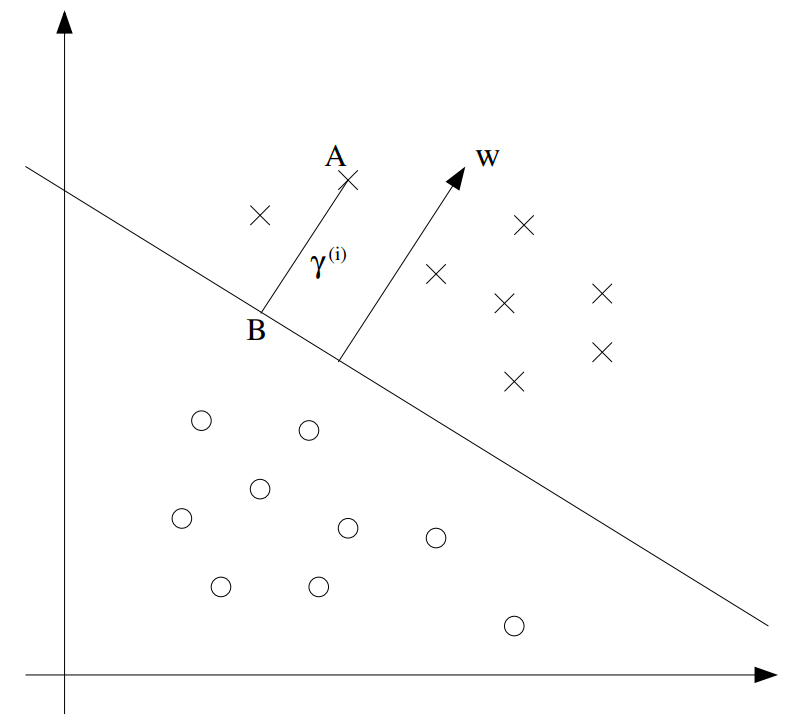
\includegraphics[width=0.5\linewidth]{figs/svm_geo_margin.png}
\end{figure}

图中显示了与 $(w,b)$ 对应的决策边界以及向量 $w$。注意 $w$ 与分隔超平面正交(呈 $90^\circ$ 角)(您应该说服自己确实如此)。 考虑 A 点,它代表标记为 $y^{(i)}=1$ 的某个训练样本的输入 $x^{(i)}$。它到决策边界的距离 $\gamma^{(i)}$ 由线段 AB 给出。

如何找到 $\gamma^{(i)}$ 的值?$w/||w||$ 是一个单位长度向量,方向与 $w$ 相同。由于 A 代表 $x^{(i)}$,因此可以发现点 B 由 $x^{(i)} - \gamma^{(i)} \cdot w/||w||$ 给出。但这个点位于决策边界上,而决策边界上的所有点 $x$ 都满足方程 $w^T x + b = 0$。因此,
\[
    w^T \left( x^{(i)} - \gamma^{(i)} \frac{w}{||w||} \right) + b = 0.
\]
解出 $\gamma^{(i)}$ 得到
\[
    \gamma^{(i)} = \frac{w^T x^{(i)} + b}{||w||} = \left(\frac{w}{||w||}\right)^T x^{(i)} + \frac{b}{||w||}.
\]
这是针对图中 A 点处正训练样本的情况推导的,其中位于决策边界的“正”侧是好的。更一般地,定义 $(w,b)$ 相对于训练样本 $(x^{(i)}, y^{(i)})$ 的几何间隔为
\[
    \gamma^{(i)} = y^{(i)} \left( \left(\frac{w}{||w||}\right)^T x^{(i)} + \frac{b}{||w||} \right).
\]

注意,如果 $||w|| = 1$,那么函数间隔等于几何间隔——这提供了一种关联这两种不同间隔概念的方式。此外,几何间隔对于参数的缩放是不变的;也就是说,如果用 $2w$ 和 $2b$ 替换 $w$ 和 $b$,那么几何间隔不会改变。这在后面会很有用。具体来说,由于参数缩放的这种不变性,在试图拟合 $w$ 和 $b$ 到训练数据时,可以在不改变任何重要内容的情况下对 $w$ 施加任意缩放约束;例如,可以要求 $||w|| = 1$,或者 $|w_1| = 5$,或者 $|w_1 + b| + |w_2| = 2$,并且这些都可以通过缩放 $w$ 和 $b$ 简单地满足。

最后,给定一个训练集 $S = \{(x^{(i)}, y^{(i)}); i = 1, \dots, n\}$,还定义 $(w,b)$ 相对于 $S$ 的几何间隔为各个训练样本的几何间隔中的最小值:
\[
    \gamma = \min_{i=1,\dots,n} \gamma^{(i)}.
\]

\section{最优间隔分类器 (选读)}

给定一个训练集,从之前的讨论来看,一个自然期望是找到一个决策边界,使其几何间隔最大化,因为这将反映一组在训练集上非常确信的预测,并且其能很好地“拟合”训练数据。具体来说,这将产生一个分类器,它用一个“间隔”(几何间隔)来分隔正训练样本和负训练样本。

目前,假设给定一个线性可分的训练集;也就是说,可以通过某个分隔超平面来分隔正样本和负样本。如何找到能实现最大几何间隔的那个呢?可以提出以下优化问题:
\begin{align*}
    \max_{\gamma, w, b} \quad &\gamma\\
    \text{s.t.} & y^{(i)}(w^T x^{(i)} + b) \ge \gamma, \quad i = 1, \dots, n\\
    &||w|| = 1.
\end{align*}
也就是说,希望最大化 $\gamma$,约束条件是每个训练样本的函数间隔至少为 $\gamma$。此外,$||w|| = 1$ 约束确保了函数间隔等于几何间隔,因此也保证了所有几何间隔至少为 $\gamma$。因此,解决这个问题将得到 $(w,b)$,使其相对于训练集具有最大的可能几何间隔。

如果能解决上面的优化问题,任务就完成了。但是,“$||w|| = 1$” 是一个令人讨厌的(非凸)约束,并且这种问题肯定不是标准优化软件可以解决的格式。因此,尝试将问题转换为更友好的形式。考虑:
\begin{align*}
    \max_{\gamma, w, b} \quad &\frac{\hat\gamma}{||w||}\\
    \text{s.t.} \quad & y^{(i)}(w^T x^{(i)} + b) \ge \hat\gamma, \quad i = 1, \dots, n
\end{align*}
这里,要最大化 $\hat{\gamma}/||w||$,约束条件是所有函数间隔至少为 $\hat{\gamma}$。由于几何间隔和函数间隔通过 $\gamma = \hat{\gamma}/||w||$ 相关,这将得到想要的答案。此外,摆脱了不喜欢的 $||w|| = 1$ 约束。缺点是现在有一个令人讨厌的(还是非凸的)目标函数 $\frac{\hat{\gamma}}{||w||}$;而且,仍然没有现成的软件可以解决这种形式的优化问题。

再想想。回想之前关于可以在不改变任何内容的情况下对 $w$ 和 $b$ 添加任意缩放约束的讨论。这是现在要使用的关键思想。引入缩放约束,使得 $(w,b)$ 相对于训练集的函数间隔必须为 1:
\[
    \hat{\gamma} = 1.
\]
由于将 $w$ 和 $b$ 乘以某个常数会导致函数间隔也乘以相同的常数,这确实是一个缩放约束,并且可以通过缩放 $w, b$ 来满足。将其代入上面的问题,并注意到最大化 $\hat{\gamma}/||w|| = 1/||w||$ 等价于最小化 $||w||^2$,现在有了以下优化问题:
\begin{align*}
    \min_{w, b} \quad &\frac{1}{2}||w||^2\\
    \text{s.t.} \quad & y^{(i)}(w^T x^{(i)} + b) \ge \hat\gamma, \quad i = 1, \dots, n
\end{align*}

现在已经将问题转换成可以有效求解的形式。上述问题是一个具有凸二次目标函数和线性约束的优化问题。其解给出了\textbf{最优间隔分类器 (optimal margin classifier)}。可以使用商用二次规划(QP)代码来解决此优化问题\footnote{您可能熟悉线性规划,它解决具有目标函数和约束均是线性的优化问题。QP 软件也广泛可用,它允许具有凸二次目标函数和线性约束。}。

虽然可以称此问题已解决,但下文会进一步讨论拉格朗日对偶性。这将导出优化问题的对偶形式,使得我们可以应用核函数让最优间隔分类器在极高维空间中高效工作。对偶形式还将允许推导出一种求解上述优化问题的高效算法,该算法通常比通用 QP 软件表现更好。

\section{拉格朗日对偶性 (选读)}

暂时搁置支持向量机和最大间隔分类器,讨论如何解决带约束的优化问题。

考虑以下形式的问题:
\begin{align*}
    \min_w \quad &f(w)\\
    \text{s.t.} \quad &h_i(w)=0,\quad i=1,\dots,l.
\end{align*}
一些读者可能还记得如何使用拉格朗日乘数法来解决此问题。(如果以前没有见过,不用担心。)在此方法中,定义\textbf{拉格朗日函数 (Lagrangian)} 为
\[
    \mathcal{L}(w, \beta) = f(w) + \sum_{i=1}^l \beta_i h_i(w)
\]
这里,$\beta_i$ 称为\textbf{拉格朗日乘数 (Lagrange multipliers)}。然后找到 $\mathcal{L}$ 的偏导数并将其设为零:
\[
    \frac{\partial \mathcal{L}}{\partial w_i} = 0; \quad \frac{\partial \mathcal{L}}{\partial \beta_i} = 0,
\]
并求解 $w$ 和 $\beta$。

在本节中,将此推广到可能包含不等式约束和等式约束的优化问题。由于时间限制,无法在本课程中充分论述拉格朗日对偶性理论\footnote{对学习更多关于此主题感兴趣的读者,建议阅读,例如,R. T. Rockafeller (1970), Convex Analysis, Princeton University Press.},但将给出主要思想和结果,并将其应用于最优间隔分类器的优化问题。

考虑以下问题,将其称为\textbf{原始 (primal)} 优化问题:

\begin{align*}
    \min_w \quad &f(w)\\
    \text{s.t.} \quad &g_i(w)\leq 0, \quad i=1,\dots,k\\
    \quad &h_i(w)=0, \quad i=1,\dots,l.
\end{align*}
为了解决它,首先定义\textbf{广义拉格朗日函数 (generalized Lagrangian)}:
\[
    \mathcal{L}(w, \alpha, \beta) = f(w) + \sum_{i=1}^k \alpha_i g_i(w) + \sum_{i=1}^l \beta_i h_i(w).
\]
这里,$\alpha_i$ 和 $\beta_i$ 是拉格朗日乘数。考虑以下量
\[
    \theta_{\mathcal{P}}(w) = \max_{\alpha, \beta: \alpha_i \ge 0} \mathcal{L}(w, \alpha, \beta).
\]
这里,下标 “$\mathcal{P}$” 代表 “原始”。给定某个 $w$。如果 $w$ 违反任何原始约束(即,对于某个 $i$,要么 $g_i(w) > 0$ 要么 $h_i(w) \ne 0$),那么应该能够验证
\begin{align}
    \theta_{\mathcal{P}}(w) &= \max_{\alpha, \beta: \alpha_i \ge 0} f(w) + \sum_{i=1}^k \alpha_i g_i(w) + \sum_{i=1}^l \beta_i h_i(w) \label{eq:6.1} \\
    &= \infty. \label{eq:6.2}
\end{align}
反之,如果约束对于某个特定的 $w$ 值确实满足,那么 $\theta_{\mathcal{P}}(w) = f(w)$。因此,
\[
    \theta_{\mathcal{P}}(w) = \begin{cases} f(w) & \text{若 } w \text{ 满足原始约束} \\ \infty & \text{其他情况}. \end{cases}
\]
因此,对于满足原始约束的所有 $w$ 值,$\theta_{\mathcal{P}}$ 取与问题中目标函数相同的值,如果违反约束,则为正无穷大。因此,如果考虑最小化问题
\[
    \min_w \theta_{\mathcal{P}}(w) = \min_w \max_{\alpha, \beta: \alpha_i \ge 0} \mathcal{L}(w, \alpha, \beta),
\]
可以看出它与原始问题相同(即,具有与原始问题相同的解)。为了后续使用,还将目标函数的最优值定义为 $p^* = \min_w \theta_{\mathcal{P}}(w)$;将其称为原始问题的\textbf{值 (value)}。

现在,考察一个稍微不同的问题。定义
\[
    \theta_{\mathcal{D}}(\alpha, \beta) = \min_w \mathcal{L}(w, \alpha, \beta).
\]
这里,下标 “$\mathcal{D}$” 代表 “对偶”。注意,在 $\theta_{\mathcal{P}}$ 的定义中,关于 $\alpha, \beta$ 进行优化(最大化),而这里关于 $w$ 进行最小化。

现在可以提出\textbf{对偶 (dual)} 优化问题:
\[
    \max_{\alpha, \beta: \alpha_i \ge 0} \theta_{\mathcal{D}}(\alpha, \beta) = \max_{\alpha, \beta: \alpha_i \ge 0} \min_w \mathcal{L}(w, \alpha, \beta).
\]
这与上面显示的原始问题完全相同,只是 “max” 和 “min” 的顺序现在交换了。将对偶问题目标函数的最优值定义为 $d^* = \max_{\alpha, \beta: \alpha_i \ge 0} \theta_{\mathcal{D}}(w)$。

原始问题和对偶问题如何关联?很容易证明
\[
    d^* = \max_{\alpha, \beta: \alpha_i \ge 0} \min_w \mathcal{L}(w, \alpha, \beta) \le \min_w \max_{\alpha, \beta: \alpha_i \ge 0} \mathcal{L}(w, \alpha, \beta) = p^*.
\]
(您应该自己证明这一点;这源自函数 “max min” 总是小于或等于 “min max”。)然而,在某些条件下,将有
\[
    d^* = p^*,
\]
这样就可以求解对偶问题来代替原始问题。来看看这些条件是什么。

假设 $f$ 和 $g_i$ 是凸函数\footnote{当 $f$ 具有 Hessian 矩阵时,当且仅当 Hessian 矩阵是半正定时,它是凸的;类似地,所有线性(和仿射)函数也是凸的。(函数 $f$ 也可以在不可微的情况下是凸的,但这里不需要那些更一般的凸性定义。)},并且 $h_i$ 是仿射函数\footnote{即,存在 $a_i, b_i$,使得 $h_i(w) = a_i^T w + b_i$。“仿射”的意思与线性相同,只是允许额外的截距项 $b_i$。}。进一步假设约束 $g_i$ 是(严格)可行的;这意味着存在某个 $w$ 使得对于所有 $i$,都有 $g_i(w) < 0$。

在上述假设下,必然存在 $w^*, \alpha^*, \beta^*$,使得 $w^*$ 是原始问题的解,$\alpha^*, \beta^*$ 是对偶问题的解,并且 $p^* = d^* = \mathcal{L}(w^*, \alpha^*, \beta^*)$。此外,$w^*, \alpha^*$ 和 $\beta^*$ 满足 \textbf{Karush-Kuhn-Tucker (KKT) 条件},如下:
\begin{align}
    \frac{\partial}{\partial w_i} \mathcal{L}(w^*, \alpha^*, \beta^*) &= 0, \quad i = 1, \dots, d \label{eq:6.3} \\
    \frac{\partial}{\partial \beta_i} \mathcal{L}(w^*, \alpha^*, \beta^*) &= 0, \quad i = 1, \dots, l \label{eq:6.4} \\
    \alpha_i^* g_i(w^*) &= 0, \quad i = 1, \dots, k \label{eq:6.5} \\
    g_i(w^*) &\le 0, \quad i = 1, \dots, k \label{eq:6.6} \\
    \alpha^* &\ge 0, \quad i = 1, \dots, k \label{eq:6.7}
\end{align}
此外,如果某个 $w^*, \alpha^*, \beta^*$ 满足 KKT 条件,那么它也是原始问题和对偶问题的解。

请注意方程 (\ref{eq:6.5}),它被称为 KKT \textbf{对偶互补性条件 (dual complementarity)}。具体来说,这意味着如果 $\alpha_i^* > 0$,那么 $g_i(w^*) = 0$。(即,“$g_i(w) \le 0$” 约束是\textbf{活跃 (active)} 的,意味着它以等式而不是不等式成立。)稍后,这将是证明 SVM 只有少量“支持向量”的关键;KKT 对偶互补性条件也将为讨论 SMO 算法时提供收敛性测试。

\section{最优间隔分类器:对偶形式 (选读)}

\textcolor{blue}{注:}\textit{优化问题 \eqref{eq:primal_opt} 与优化问题 \eqref{eq:dual_opt} 的等价性,以及方程 \eqref{eq:dual_relation} 中原始变量和对偶变量之间的关系是本节最重要的收获。}

前面,提出了以下寻找最优间隔分类器的问题(原始)优化问题:
\begin{align}
    \min_{w,b} \quad &\frac{1}{2}\|w\|^2 \label{eq:primal_opt}\\
    \text{s.t.} \quad &y^{(i)}(w^T x^{(i)} + b) \ge 1, \quad i = 1, \dots, n \notag
\end{align}
可以将约束写成
\[
    g_i(w) = -y^{(i)}(w^T x^{(i)} + b) + 1 \le 0.
\]
每个训练样本都有一个这样的约束。注意,根据 KKT 对偶互补性条件,只有当训练样本的功能间隔恰好等于 1 时(即,对应于满足等式 $g_i(w) = 0$ 的约束),$\alpha_i$ 才大于 0。考虑下图中,其中实线表示最大间隔分离超平面。

\begin{figure}[H]
    \centering
    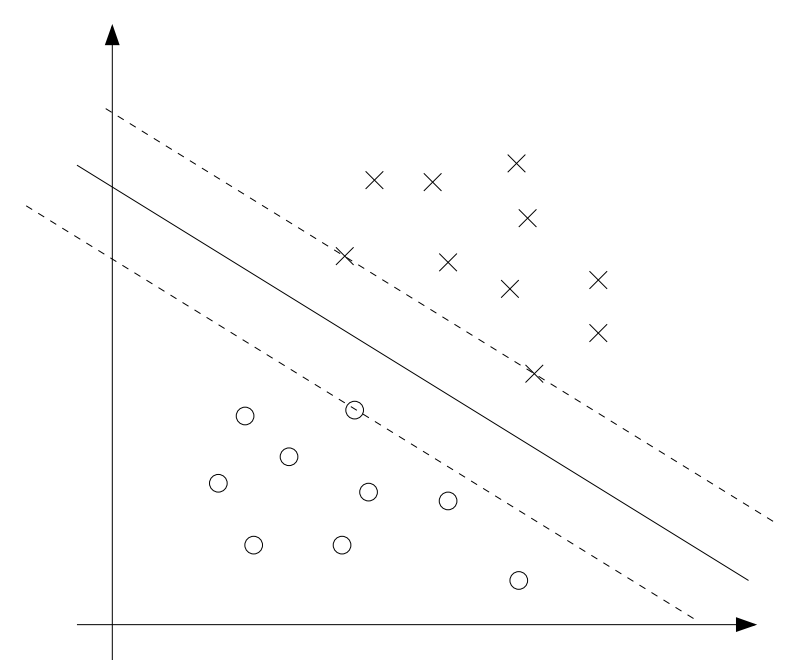
\includegraphics[width=0.5\linewidth]{figs/svm_max_margin.png}
\end{figure}

间隔最小的点恰好是离决策边界最近的点;在这里,这三个点(一个负样本和两个正样本)位于平行于决策边界的虚线上。因此,只有这三个 $\alpha_i$(即,对应于这三个训练样本的 $\alpha_i$)在最优解处非零。这三个点被称为该问题中的\textbf{支持向量 (support vectors)}。支持向量的数量可以远小于训练集的大小,这一事实将在稍后有用。

接下来,在推导对偶形式问题时,需要注意的一个关键思想是,我们将尝试仅使用内积 $\langle x^{(i)}, x^{(j)} \rangle$(将其视为输入特征空间中点之间的 $(x^{(i)})^T x^{(j)}$)来编写算法。算法能够用这些内积表达的事实是应用核技巧的关键。

构建优化问题的拉格朗日函数为:
\begin{equation}
    \mathcal{L}(w, b, \alpha) = \frac{1}{2}\|w\|^2 - \sum_{i=1}^n \alpha_i [y^{(i)}(w^T x^{(i)} + b) - 1]. \label{eq:la_opt}
\end{equation}
注意,只有“$\alpha_i$”而没有“$\beta_i$”拉格朗日乘子,因为问题只有不等式约束。

继续推导问题的对偶形式。为此,需要首先对固定的 $\alpha$ 最小化 $\mathcal{L}(w, b, \alpha)$ 关于 $w$ 和 $b$,以得到 $\theta_D$。方法是将 $\mathcal{L}$ 关于 $w$ 和 $b$ 的导数设为零。得到:
\[
    \nabla_w \mathcal{L}(w, b, \alpha) = w - \sum_{i=1}^n \alpha_i y^{(i)} x^{(i)} = 0
\]
这意味着
\begin{equation}
    w = \sum_{i=1}^n \alpha_i y^{(i)} x^{(i)}. \label{eq:dual_relation}
\end{equation}
关于 $b$ 的导数,得到
\begin{equation}
    \frac{\partial}{\partial b} \mathcal{L}(w, b, \alpha) = \sum_{i=1}^n \alpha_i y^{(i)} = 0. \label{eq:6.11}
\end{equation}
将式 \eqref{eq:dual_relation} 中 $w$ 的定义代入拉格朗日函数 \eqref{eq:la_opt},并简化,得到
\[
    \mathcal{L}(w, b, \alpha) = \sum_{i=1}^n \alpha_i - \frac{1}{2} \sum_{i,j=1}^n y^{(i)} y^{(j)} \alpha_i \alpha_j (x^{(i)})^T x^{(j)} - b \sum_{i=1}^n \alpha_i y^{(i)}.
\]
但根据式 \eqref{eq:6.11},最后一项必须为零,所以得到
\[
    \mathcal{L}(w, b, \alpha) = \sum_{i=1}^n \alpha_i - \frac{1}{2} \sum_{i,j=1}^n y^{(i)} y^{(j)} \alpha_i \alpha_j (x^{(i)})^T x^{(j)}.
\]
回想一下,通过对 $\mathcal{L}$ 关于 $w$ 和 $b$ 进行最小化,得到了上面的方程。将其与约束 $\alpha_i \ge 0$(始终存在)和约束 \eqref{eq:6.11} 结合,得到以下对偶优化问题:
\begin{align}
    \max_\alpha \quad &W(\alpha) = \sum_{i=1}^n \alpha_i - \frac{1}{2} \sum_{i,j=1}^n y^{(i)} y^{(j)} \alpha_i \alpha_j \langle x^{(i)}, x^{(j)} \rangle \label{eq:dual_opt} \\
    \text{s.t.} \quad & \alpha_i \ge 0, \quad i=1,\dots,n \notag\\
     & \sum_{i=1}^n \alpha_i y^{(i)} = 0. \notag
\end{align}

还应该能够验证 $p^* = d^*$ 所需的条件以及 KKT 条件(式 \eqref{eq:6.3}-\eqref{eq:6.7})在我们的优化问题里确实满足。因此,可以通过求解对偶问题来求解原问题。具体而言,在上述对偶问题中,这是一个最大化问题,其中的参数是 $\alpha_i$。稍后将讨论用于求解对偶问题的具体算法,但如果确实能够求解它(即找到使 $W(\alpha)$ 最大化且满足约束的 $\alpha$),那么就可以使用式 \eqref{eq:dual_relation} 回过头来找到最优的 $w$ 作为 $\alpha$ 的函数。找到 $w^*$ 后,通过考虑原问题,也很容易找到截距项 $b$ 的最优值,如下所示:
\begin{equation}
    b^* = - \frac{\max_{i:y^{(i)}=-1} w^{*T} x^{(i)} + \min_{i:y^{(i)}=1} w^{*T} x^{(i)}}{2}. \label{eq:6.13}
\end{equation}
(可以自行验证一下此处的正确性。)

继续之前,再仔细看看式 \eqref{eq:dual_relation},它给出了 $w$ 的最优值(以最优 $\alpha$ 表示)。假设已经用训练集拟合了模型参数,现在想对新的输入点 $x$ 进行预测。然后计算 $w^T x + b$,并且当且仅当该值大于零时预测 $y=1$。但是使用 \eqref{eq:dual_relation},该值也可以写成:
\begin{align}
    w^T x + b &= \left(\sum_{i=1}^n \alpha_i y^{(i)} x^{(i)}\right)^T x + b \\
    &= \sum_{i=1}^n \alpha_i y^{(i)} \langle x^{(i)}, x \rangle + b. \label{eq:6.15}
\end{align}
因此,如果找到了 $\alpha_i$,为了进行预测,必须计算一个仅取决于 $x$ 与训练集中的点之间的内积的值。此外,之前已经看到,除了支持向量对应的 $\alpha_i$ 外,其他所有 $\alpha_i$ 都将为零。因此,上面求和中的许多项将为零,并且实际上只需要计算 $x$ 与支持向量(通常数量很少)之间的内积,以便计算 \eqref{eq:6.15} 并进行预测。

通过研究优化问题的对偶形式,对问题的结构获得了重要的见解,并且还能够仅以内积形式编写整个算法。在下一节中,将利用这一特性将核函数应用于分类问题。由此产生的算法,\textbf{支持向量机 (support vector machines)},将能够在非常高维的空间中高效学习。

\section{正则化与非线性可分情况 (选读)}

目前为止介绍的支持向量机推导假设数据是线性可分的。虽然通过 $\phi$ 将数据映射到高维特征空间通常会增加数据可分的可能性,但不能保证总是如此。此外,在某些情况下,找到一个分离超平面并非完全符合期望,因为它可能对离群点敏感。例如,下面左图显示了一个最优间隔分类器,当在左上方区域(右图)添加一个离群点时,决策边界会发生剧烈变化,并且得到的分类器的间隔会小得多。

\begin{figure}[H]
    \centering
    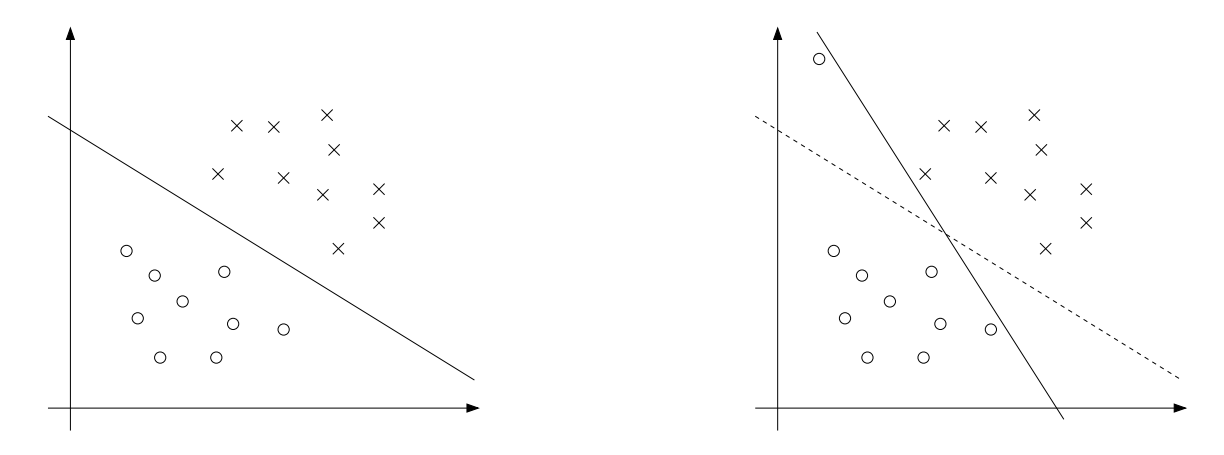
\includegraphics[width=0.93\linewidth]{figs/svm_regularization.png}
\end{figure}

为了使算法也适用于非线性可分数据集并降低对离群点的敏感度,我们重新构建了优化问题(使用 $\ell_1$ \textbf{正则化 (regularization)}),如下所示:
\begin{align*}
    \min_{\gamma,w,b} \quad& \frac{1}{2}\|w\|^2 + C \sum_{i=1}^n \xi_i \\
    \text{s.t.} \quad& y^{(i)}(w^T x^{(i)} + b) \ge 1 - \xi_i, \quad i=1,\dots,n \\
    &\xi_i \ge 0, \quad i=1,\dots,n.
\end{align*}
因此,现在允许存在(函数)间隔小于 1 的样本,如果一个样本的函数间隔为 $1-\xi_i$(其中 $\xi_i > 0$),那么目标函数会增加 $C\xi_i$ 的代价。参数 $C$ 控制了两个目标之间的相对权重:使 $\|w\|^2$ 小(如前面所述,这会使间隔大)以及确保大多数样本的函数间隔至少为 1。

与之前一样,可以构建拉格朗日函数:
\[
    \mathcal{L}(w, b, \xi, \alpha, r) = \frac{1}{2} w^T w + C \sum_{i=1}^n \xi_i - \sum_{i=1}^n \alpha_i [y^{(i)}(w^T x^{(i)} + b) - 1 + \xi_i] - \sum_{i=1}^n r_i \xi_i.
\]
这里,$\alpha_i$ 和 $r_i$ 是拉格朗日乘子(约束为 $\ge 0$)。将不再详细推导对偶问题,但在像之前一样将关于 $w$ 和 $b$ 的导数设为零,然后代入并简化后,得到问题的对偶形式:
\begin{align*}
    \max{\alpha} \quad& W(a)=\sum_{i=1}^{n}a_i - \frac12 \sum_{i,j=1}^n y^{(i)}y^{(j)}\alpha_i\alpha_j\langle x^{(i)}x^{(j)} \rangle \\
    \text{s.t.} \quad& 0\le \alpha_i\le C, \quad i=1,\dots,n \\
    &\sum_{i=1}^{n}\alpha_i y^{(i)}=0.
\end{align*}

与之前一样,同样有 $w$ 可以表示为 $\alpha_i$ 的函数,如式 \eqref{eq:dual_relation} 所示,因此在求解对偶问题后,可以继续使用式 \eqref{eq:6.15} 进行预测。注意,令人惊讶的是,在添加 $\ell_1$ 正则化后,对偶问题唯一的改变是原先的约束 $0 \le \alpha_i$ 现在变成了 $0 \le \alpha_i \le C$。对 $b^*$ 的计算也必须进行修改(式 \eqref{eq:6.13} 不再有效);请参阅下一节中的注释或 Platt 的论文。

此外,KKT 对偶互补条件(在下一节中将用于测试 SMO 算法的收敛性)为:
\begin{align}
    \alpha_i = 0 &\Rightarrow y^{(i)}(w^T x^{(i)} + b) \ge 1 \label{eq:6.16} \\
    \alpha_i = C &\Rightarrow y^{(i)}(w^T x^{(i)} + b) \le 1 \label{eq:6.17} \\
    0 < \alpha_i < C &\Rightarrow y^{(i)}(w^T x^{(i)} + b) = 1. \label{eq:6.18}
\end{align}
现在,剩下的就是给出一个实际求解对偶问题的算法,这将在下一节中进行。

\section{SMO 算法 (选读)}

序列最小化 (sequential minimal optimization, SMO) 算法,由 John Platt 提出,提供了一种有效求解由 SVM 推导得到的对偶问题的方法。部分是为了引出 SMO 算法,部分是因为它本身很有趣,让我们先再进行一次岔开讨论,谈谈坐标上升算法。

\subsection{坐标上升}

考虑尝试求解无约束优化问题
\[
    \max_\alpha W(\alpha_1, \alpha_2, \dots, \alpha_n).
\]
这里,将 $W$ 视为参数 $\alpha_i$ 的某个函数,暂时忽略这个问题与支持向量机之间的任何关系。之前已经见过两种优化算法:梯度上升和牛顿法。这里要考虑的新算法称为\textbf{坐标上升 (coordinate ascent)}:

循环直到收敛: \{

    $\quad\quad$对于 $i=1,\dots,n,$ \{
        \[
            \alpha_i := \arg\max_{\hat a_i} W(\alpha_1,\dots,\alpha_{i-1},\hat{\alpha_i},\alpha_{i+1},\dots,\alpha_n).
        \]
        
    $\quad\quad$\}

\}

因此,在该算法的最内层循环中,将固定除某个 $\alpha_i$ 之外的所有变量,并仅针对参数 $\alpha_i$ 重新优化 $W$。在该方法此处介绍的版本中,内层循环按 $\alpha_1, \alpha_2, \dots, \alpha_n, \alpha_1, \alpha_2, \dots$ 的顺序重新优化变量。(更复杂的版本可以选择其他顺序;例如,可以根据期望哪个变量能使 $W(\alpha)$ 增加最大来选择下一个要更新的变量。)

当函数 $W$ 的形式恰好使得内层循环中的 “arg max” 可以高效执行时,坐标上升可以是一个相当高效的算法。这里是坐标上升算法的一个图例:

\begin{figure}[H]
    \centering
    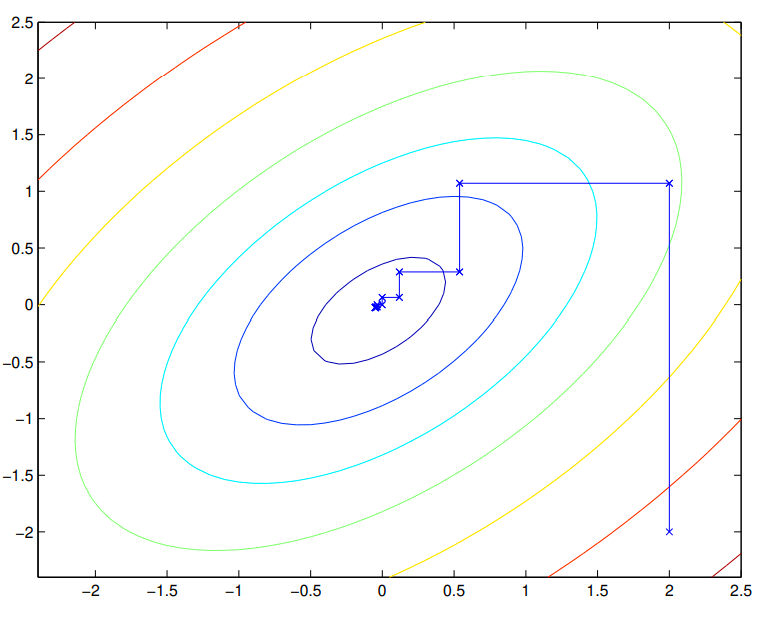
\includegraphics[width=0.5\linewidth]{figs/svm_coordinate_ascent.png}
\end{figure}


图中的椭圆是我们想要优化的二次函数的等高线。坐标上升从 $(2, -2)$ 初始化,图中绘制了它通往全局最大值的路径。注意到在每一步,坐标上升都沿着与一个坐标轴平行的方向前进,因为每次只优化一个变量。

\subsection{SMO}

通过概述 SMO 算法的推导来结束对支持向量机的讨论。

这是我们想要解决的(对偶)优化问题:
\begin{align}
    \max_\alpha \quad &W(\alpha) = \sum_{i=1}^n \alpha_i - \frac{1}{2} \sum_{i,j=1}^n y^{(i)} y^{(j)} \alpha_i \alpha_j \langle x^{(i)}, x^{(j)} \rangle \\
    \text{s.t.} \quad &0 \le \alpha_i \le C, \quad i=1,\dots,n \label{eq:6.20}\\
    &\sum_{i=1}^n \alpha_i y^{(i)} = 0. \label{eq:6.21}
\end{align}

假设我们有一组满足约束 (\eqref{eq:6.20}-\eqref{eq:6.21}) 的 $\alpha_i$。现在,假设我们固定 $\alpha_2, \dots, \alpha_n$,并进行坐标上升步骤,关于 $\alpha_1$重新优化目标函数。能取得任何进展吗?答案是否定的,因为约束 \eqref{eq:6.21} 确保
\[
    \alpha_1 y^{(1)} = - \sum_{i=2}^n \alpha_i y^{(i)}.
\]

或者,通过将两边乘以 $y^{(1)}$,我们等价地得到
\[
    \alpha_1 = -y^{(1)} \sum_{i=2}^n \alpha_i y^{(i)}.
\]
(这一步使用了 $y^{(1)} \in \{-1, 1\}$ 的事实,因此 $(y^{(1)})^2 = 1$。)因此,$\alpha_1$ 完全由其他 $\alpha_i$ 确定,如果固定 $\alpha_2, \dots, \alpha_n$,那么在不违反优化问题中的约束 \eqref{eq:6.21} 的情况下,无法对 $\alpha_1$ 进行任何改变。

因此,如果想要更新一些 $\alpha_i$,必须同时更新至少两个,以便保持约束得到满足。这促使了 SMO 算法,其简单来说就是以下步骤:

\begin{samepage}
重复直到收敛 \{
\vspace{-0.5em}
\begin{enumerate}
\setlength{\itemindent}{2em}
    \item 选择一对 $\alpha_i$ 和 $\alpha_j$ 进行下一次更新(使用启发式方法来选择能够最大程度接近全局最大值的两个变量)。
    \item 在保持所有其他 $\alpha_k$ ($k \ne i, j$) 固定的情况下,重新优化 $W(\alpha)$ 关于 $\alpha_i$ 和 $\alpha_j$。
\end{enumerate}
$\quad\quad$\}
\end{samepage}

为了测试该算法的收敛性,可以检查 KKT 条件(式 \eqref{eq:6.16}-\eqref{eq:6.18})是否在某个 $\textit{容差 (tol)}$ 内得到满足。这里,容差是收敛容差参数,通常设置为 0.01 到 0.001。(详细信息请参阅论文和伪代码。)

SMO 算法高效的关键原因在于 $\alpha_i, \alpha_j$ 的更新可以非常高效地计算。现在简要概述推导高效更新的主要思路。

假设当前有一组满足约束 (\eqref{eq:6.20}-\eqref{eq:6.21}) 的 $\alpha_i$,并且假设决定固定 $\alpha_3, \dots, \alpha_n$,并重新优化 $W(\alpha_1, \alpha_2, \dots, \alpha_n)$ 关于 $\alpha_1$ 和 $\alpha_2$(受约束限制)。根据 \eqref{eq:6.21},我们要求
\[
    \alpha_1 y^{(1)} + \alpha_2 y^{(2)} = - \sum_{i=3}^n \alpha_i y^{(i)}.
\]
由于右侧是固定的(因为已经固定了 $\alpha_3, \dots, \alpha_n$),可以将其记为某个常数 $\zeta$:
\begin{equation}
    \alpha_1 y^{(1)} + \alpha_2 y^{(2)} = \zeta. \label{eq:6.22}
\end{equation}
因此,可以将 $\alpha_1$ 和 $\alpha_2$ 的约束可视化如下:

\begin{figure}[H]
    \centering
    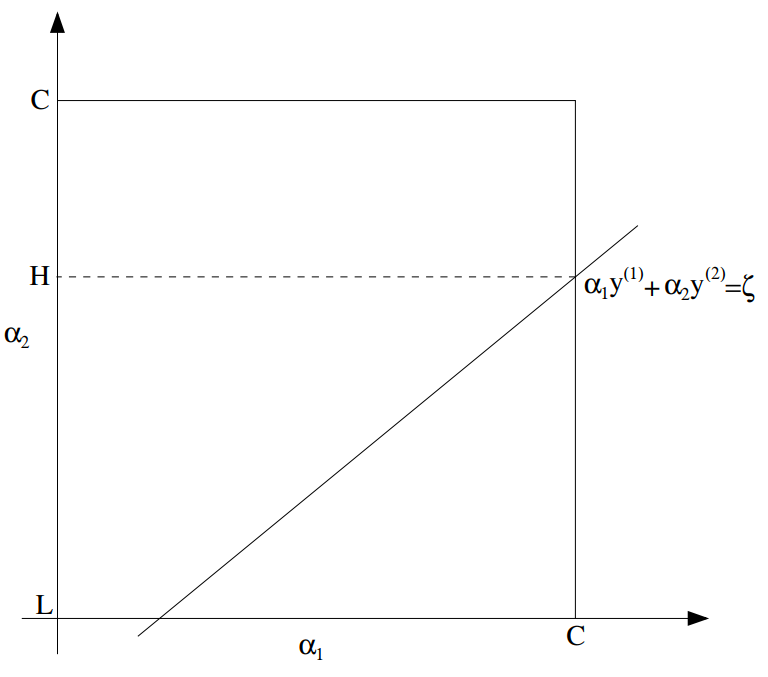
\includegraphics[width=0.5\linewidth]{figs/svm_smo_constraint.png}
\end{figure}

从约束 \eqref{eq:6.20} 中,我们知道 $\alpha_1$ 和 $\alpha_2$ 必须位于所示的盒子 $[0, C] \times [0, C]$ 内。还绘制了直线 $\alpha_1 y^{(1)} + \alpha_2 y^{(2)} = \zeta$,我们知道 $\alpha_1$ 和 $\alpha_2$ 必须位于该直线上。另外注意,从这些约束中,我们知道 $L \le \alpha_2 \le H$;否则,$(\alpha_1, \alpha_2)$ 无法同时满足盒子约束和直线约束。在此示例中,$L=0$。但这取决于直线 $\alpha_1 y^{(1)} + \alpha_2 y^{(2)} = \zeta$ 的样子,情况并非总是如此;更普遍地,对于 $\alpha_2$ 的允许值,会有一个下界 $L$ 和一个上界 $H$,以确保 $\alpha_1, \alpha_2$ 位于盒子 $[0, C] \times [0, C]$ 内。

使用方程 \eqref{eq:6.22},我们还可以将 $\alpha_1$ 写成 $\alpha_2$ 的函数:
\[
    \alpha_1 = (\zeta - \alpha_2 y^{(2)}) y^{(1)}.
\]
(请自行验证此推导;我们再次使用了 $y^{(1)} \in \{-1, 1\}$ 的事实,因此 $(y^{(1)})^2 = 1$。)因此,目标函数 $W(\alpha)$ 可以写成
\[
    W(\alpha_1, \alpha_2, \dots, \alpha_n) = W((\zeta - \alpha_2 y^{(2)}) y^{(1)}, \alpha_2, \dots, \alpha_n).
\]
将 $\alpha_3, \dots, \alpha_n$ 视为常数,您应该能够验证这是关于 $\alpha_2$ 的二次函数。也就是说,这也可以表示为 $a\alpha_2^2 + b\alpha_2 + c$ 的形式,其中 $a, b, c$ 是适当的常数。如果忽略“盒子”约束 \eqref{eq:6.20}(或等价地,忽略 $L \le \alpha_2 \le H$),那么我们可以通过将其导数设为零并求解来轻松最大化此二次函数。我们将令 $\alpha_2^{\text{new,unclipped}}$ 表示由此产生的 $\alpha_2$ 值。您还应该能够说服自己,如果改为最大化关于 $\alpha_2$ 的 $W$,但受盒子约束限制,那么可以通过简单地取 $\alpha_2^{\text{new,unclipped}}$ 并将其“剪裁”到$[L, H]$ 区间内,得到
\[
    \alpha_2^{\text{new}} = \begin{cases}
        H & \text{若}\  \alpha_2^{\text{new,unclipped}} > H \\
        \alpha_2^{\text{new,unclipped}} & \text{若}\  L \le \alpha_2^{\text{new,unclipped}} \le H \\
        L & \text{若}\  \alpha_2^{\text{new,unclipped}} < L
    \end{cases}
\]
最后,找到 $\alpha_2^{\text{new}}$ 后,可以使用方程 \eqref{eq:6.22} 返回并找到 $\alpha_1^{\text{new}}$ 的最优值。

还有一些细节非常简单,但我们将留给您自己在 Platt 的论文中阅读:一个是用于选择下一个要更新的 $\alpha_i, \alpha_j$ 的启发式方法的选择;另一个是 SMO 算法运行时如何更新 $b$。